% Options for packages loaded elsewhere
% Options for packages loaded elsewhere
\PassOptionsToPackage{unicode,hidelinks}{hyperref}
\PassOptionsToPackage{hyphens}{url}
%
\documentclass[
  swedish,
  11pt,
  a4paper,
  DIV=11,
  numbers=noendperiod,
  twoside,
  open=any]{scrreprt}
\usepackage{xcolor}
\usepackage[inner=25mm,outer=20mm,top=20mm,bottom=25mm,includeheadfoot,heightrounded]{geometry}
\usepackage{amsmath,amssymb}
\setcounter{secnumdepth}{2}
\usepackage{iftex}
\ifPDFTeX
  \usepackage[T1]{fontenc}
  \usepackage[utf8]{inputenc}
  \usepackage{textcomp} % provide euro and other symbols
\else % if luatex or xetex
  \usepackage{unicode-math} % this also loads fontspec
  \defaultfontfeatures{Scale=MatchLowercase}
  \defaultfontfeatures[\rmfamily]{Ligatures=TeX,Scale=1}
\fi
\usepackage{lmodern}
\ifPDFTeX\else
  % xetex/luatex font selection
  \setmainfont[]{Latin Modern Roman}
  \setsansfont[]{Latin Modern Sans}
  \setmonofont[]{Latin Modern Mono}
  \setmathfont[]{Latin Modern Math}
\fi
% Use upquote if available, for straight quotes in verbatim environments
\IfFileExists{upquote.sty}{\usepackage{upquote}}{}
\IfFileExists{microtype.sty}{% use microtype if available
  \usepackage[]{microtype}
  \UseMicrotypeSet[protrusion]{basicmath} % disable protrusion for tt fonts
}{}
\makeatletter
\@ifundefined{KOMAClassName}{% if non-KOMA class
  \IfFileExists{parskip.sty}{%
    \usepackage{parskip}
  }{% else
    \setlength{\parindent}{0pt}
    \setlength{\parskip}{6pt plus 2pt minus 1pt}}
}{% if KOMA class
  \KOMAoptions{parskip=half}}
\makeatother
% Make \paragraph and \subparagraph free-standing
\makeatletter
\ifx\paragraph\undefined\else
  \let\oldparagraph\paragraph
  \renewcommand{\paragraph}{
    \@ifstar
      \xxxParagraphStar
      \xxxParagraphNoStar
  }
  \newcommand{\xxxParagraphStar}[1]{\oldparagraph*{#1}\mbox{}}
  \newcommand{\xxxParagraphNoStar}[1]{\oldparagraph{#1}\mbox{}}
\fi
\ifx\subparagraph\undefined\else
  \let\oldsubparagraph\subparagraph
  \renewcommand{\subparagraph}{
    \@ifstar
      \xxxSubParagraphStar
      \xxxSubParagraphNoStar
  }
  \newcommand{\xxxSubParagraphStar}[1]{\oldsubparagraph*{#1}\mbox{}}
  \newcommand{\xxxSubParagraphNoStar}[1]{\oldsubparagraph{#1}\mbox{}}
\fi
\makeatother


\usepackage{longtable,booktabs,array}
\newcounter{none} % for unnumbered tables
\usepackage{calc} % for calculating minipage widths
% Correct order of tables after \paragraph or \subparagraph
\usepackage{etoolbox}
\makeatletter
\patchcmd\longtable{\par}{\if@noskipsec\mbox{}\fi\par}{}{}
\makeatother
% Allow footnotes in longtable head/foot
\IfFileExists{footnotehyper.sty}{\usepackage{footnotehyper}}{\usepackage{footnote}}
\makesavenoteenv{longtable}
\usepackage{graphicx}
\makeatletter
\newsavebox\pandoc@box
\newcommand*\pandocbounded[1]{% scales image to fit in text height/width
  \sbox\pandoc@box{#1}%
  \Gscale@div\@tempa{\textheight}{\dimexpr\ht\pandoc@box+\dp\pandoc@box\relax}%
  \Gscale@div\@tempb{\linewidth}{\wd\pandoc@box}%
  \ifdim\@tempb\p@<\@tempa\p@\let\@tempa\@tempb\fi% select the smaller of both
  \ifdim\@tempa\p@<\p@\scalebox{\@tempa}{\usebox\pandoc@box}%
  \else\usebox{\pandoc@box}%
  \fi%
}
% Set default figure placement to htbp
\def\fps@figure{htbp}
\makeatother


% definitions for citeproc citations
\NewDocumentCommand\citeproctext{}{}
\NewDocumentCommand\citeproc{mm}{%
  \begingroup\def\citeproctext{#2}\cite{#1}\endgroup}
\makeatletter
 % allow citations to break across lines
 \let\@cite@ofmt\@firstofone
 % avoid brackets around text for \cite:
 \def\@biblabel#1{}
 \def\@cite#1#2{{#1\if@tempswa , #2\fi}}
\makeatother
\newlength{\cslhangindent}
\setlength{\cslhangindent}{1.5em}
\newlength{\csllabelwidth}
\setlength{\csllabelwidth}{3em}
\newenvironment{CSLReferences}[2] % #1 hanging-indent, #2 entry-spacing
 {\begin{list}{}{%
  \setlength{\itemindent}{0pt}
  \setlength{\leftmargin}{0pt}
  \setlength{\parsep}{0pt}
  % turn on hanging indent if param 1 is 1
  \ifodd #1
   \setlength{\leftmargin}{\cslhangindent}
   \setlength{\itemindent}{-1\cslhangindent}
  \fi
  % set entry spacing
  \setlength{\itemsep}{#2\baselineskip}}}
 {\end{list}}
\usepackage{calc}
\newcommand{\CSLBlock}[1]{\hfill\break\parbox[t]{\linewidth}{\strut\ignorespaces#1\strut}}
\newcommand{\CSLLeftMargin}[1]{\parbox[t]{\csllabelwidth}{\strut#1\strut}}
\newcommand{\CSLRightInline}[1]{\parbox[t]{\linewidth - \csllabelwidth}{\strut#1\strut}}
\newcommand{\CSLIndent}[1]{\hspace{\cslhangindent}#1}

\ifLuaTeX
\usepackage[bidi=basic,shorthands=off]{babel}
\else
\usepackage[bidi=default,shorthands=off]{babel}
\fi
\ifPDFTeX
\else
\babelfont{rm}[]{Latin Modern Roman}
\fi
\ifLuaTeX
  \usepackage{selnolig} % disable illegal ligatures
\fi


\setlength{\emergencystretch}{3em} % prevent overfull lines

\providecommand{\tightlist}{%
  \setlength{\itemsep}{0pt}\setlength{\parskip}{0pt}}



 


\AtBeginDocument{
  \setlength{\parskip}{3pt}
  \setlength{\parindent}{0pt}
  }
  
\usepackage{caption}
\captionsetup{
  font=small,
  labelfont=bf,
  textfont=normalfont,
  labelsep=colon,
  justification=raggedright,
  singlelinecheck=false
}
\KOMAoption{captions}{tableheading}
\makeatletter
\@ifpackageloaded{tcolorbox}{}{\usepackage[skins,breakable]{tcolorbox}}
\@ifpackageloaded{fontawesome5}{}{\usepackage{fontawesome5}}
\definecolor{quarto-callout-color}{HTML}{909090}
\definecolor{quarto-callout-note-color}{HTML}{0758E5}
\definecolor{quarto-callout-important-color}{HTML}{CC1914}
\definecolor{quarto-callout-warning-color}{HTML}{EB9113}
\definecolor{quarto-callout-tip-color}{HTML}{00A047}
\definecolor{quarto-callout-caution-color}{HTML}{FC5300}
\definecolor{quarto-callout-color-frame}{HTML}{acacac}
\definecolor{quarto-callout-note-color-frame}{HTML}{4582ec}
\definecolor{quarto-callout-important-color-frame}{HTML}{d9534f}
\definecolor{quarto-callout-warning-color-frame}{HTML}{f0ad4e}
\definecolor{quarto-callout-tip-color-frame}{HTML}{02b875}
\definecolor{quarto-callout-caution-color-frame}{HTML}{fd7e14}
\makeatother
\makeatletter
\@ifpackageloaded{bookmark}{}{\usepackage{bookmark}}
\makeatother
\makeatletter
\@ifpackageloaded{caption}{}{\usepackage{caption}}
\AtBeginDocument{%
\ifdefined\contentsname
  \renewcommand*\contentsname{Innehållsförteckning}
\else
  \newcommand\contentsname{Innehållsförteckning}
\fi
\ifdefined\listfigurename
  \renewcommand*\listfigurename{Figurförteckning}
\else
  \newcommand\listfigurename{Figurförteckning}
\fi
\ifdefined\listtablename
  \renewcommand*\listtablename{Tabellförteckning}
\else
  \newcommand\listtablename{Tabellförteckning}
\fi
\ifdefined\figurename
  \renewcommand*\figurename{Figur}
\else
  \newcommand\figurename{Figur}
\fi
\ifdefined\tablename
  \renewcommand*\tablename{Tabell}
\else
  \newcommand\tablename{Tabell}
\fi
}
\@ifpackageloaded{float}{}{\usepackage{float}}
\floatstyle{ruled}
\@ifundefined{c@chapter}{\newfloat{codelisting}{h}{lop}}{\newfloat{codelisting}{h}{lop}[chapter]}
\floatname{codelisting}{Lista}
\newcommand*\listoflistings{\listof{codelisting}{Listförteckning}}
\makeatother
\makeatletter
\makeatother
\makeatletter
\@ifpackageloaded{caption}{}{\usepackage{caption}}
\@ifpackageloaded{subcaption}{}{\usepackage{subcaption}}
\makeatother
\usepackage{bookmark}
\IfFileExists{xurl.sty}{\usepackage{xurl}}{} % add URL line breaks if available
\urlstyle{same}
% fallback for those not using the hyperref driver hyperxmp:
\makeatletter
\@ifundefined{xmpquote}{\newcommand{\xmpquote}[1]{#1}}{}
\makeatother
\hypersetup{
  pdftitle={Ellära},
  pdfauthor={Henrik Hallenberg},
  pdflang={sv},
  hidelinks,
  pdfcreator={LaTeX via pandoc}}


\title{Ellära}
\usepackage{etoolbox}
\makeatletter
\providecommand{\subtitle}[1]{% add subtitle to \maketitle
  \apptocmd{\@title}{\par {\large #1 \par}}{}{}
}
\makeatother
\subtitle{Kretsanalys för elektronik}
\author{Henrik Hallenberg}
\date{}
\begin{document}
\maketitle

\renewcommand*\contentsname{Innehåll}
{
\setcounter{tocdepth}{1}
\tableofcontents
}

\bookmarksetup{startatroot}

\chapter*{Förord}\label{fuxf6rord}
\addcontentsline{toc}{chapter}{Förord}

\markboth{Förord}{Förord}

Denna bok behandlar grundläggande ellära och kretsanalys med inriktning
mot elektronik.

\bookmarksetup{startatroot}

\chapter{Introduction}\label{introduction}

This is a book created from markdown and executable code.

See {[}1{]} for additional discussion of literate programming.

\bookmarksetup{startatroot}

\chapter{Summary}\label{summary}

In summary, this book has no content whatsoever.

\bookmarksetup{startatroot}

\chapter{Elektriska storheter och grundläggande
samband}\label{sec-grunder}

Elektronik handlar om att läsa av, styra och kontrollera elektriska
strömmar och spänningar. Några exempel:

\begin{itemize}
\item
  I en temperatursensor omvandlas en fysikalisk storhet (temperatur)
  till en elektrisk signal som kan läsas av en elektronisk krets.
\item
  I en förstärkare bearbetas en elektrisk signal för att göra den
  starkare genom att öka dess amplitud.
\item
  I en motor omvandlas elektrisk energi till rörelse och hastigheten
  styrs med hjälp av elektriska signaler.
\end{itemize}

För att förstå och beräkna elektriska kretsar behöver vi ett gemensamt
språk. Vi behöver kunna beskriva vad som händer, ange storheter med rätt
enheter och använda modeller som fångar kretsens viktigaste egenskaper.

I det här kapitlet introduceras elektrisk laddning, ström, potential,
spänning, resistans, konduktans och ideala källor. Med Ohms lag och
Kirchhoffs lagar får vi sedan våra första verktyg för kretsanalys.

\section*{Mål}\label{sec-grunder-mal}
\addcontentsline{toc}{section}{Mål}

\markright{Mål}

Efter kapitlet ska du kunna:

\begin{itemize}
\tightlist
\item
  förklara vad en elektrisk modell är och ge exempel på dess
  förenklingar,
\item
  beskriva elektrisk laddning och beräkna sambandet mellan laddning,
  ström och tid,
\item
  förklara skillnaden mellan potential och spänning samt använda en vald
  referenspunkt,
\item
  tolka strömriktningar, spänningspolariteter och negativa
  beräkningsresultat,
\item
  använda storheter, enheter och SI-prefix korrekt,
\item
  skilja mellan en resistor och storheten resistans samt beräkna
  resistans och konduktans,
\item
  beräkna en ledares resistans utifrån resistivitet, längd och
  tvärsnittsarea,
\item
  förklara skillnaden mellan en ideal spänningskälla och en ideal
  strömkälla,
\item
  använda Ohms lag och Kirchhoffs lagar för att lösa enkla kretsproblem,
\item
  redovisa beräkningar och kontrollera enheter, storleksordning och
  rimlighet.
\end{itemize}

\section{Elektriska kretsar och
modeller}\label{sec-grunder-elektriska-kretsar-och-modeller}

En elektrisk krets består av komponenter som är sammankopplade med
ledare. Komponenterna kan exempelvis vara spänningskällor, resistorer,
kondensatorer och transistorer.

Ett \textbf{kretsschema} visar hur komponenterna är elektriskt
sammankopplade. Det visar däremot normalt inte deras fysiska placering
eller ledningarnas verkliga längd (se Figur~\ref{fig-grunder-koppling}).

\begin{figure}

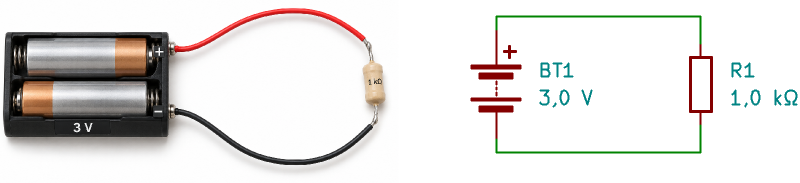
\includegraphics[width=16cm,height=\textheight,keepaspectratio]{_bilder/01-fysisk-koppling.png}

\caption{\label{fig-grunder-koppling}En sluten krets med batteri och
resistor. Samma elektriska koppling som fysisk uppkoppling (vänster)
samt som kretsschema (höger). Schemat visar anslutningarna, inte
komponenternas fysiska placering. I schemat kan referensbeteckning och
värde för respektive komponent anges, t.ex.
\(R_1 = 1{,}0\,\mathrm{k}\Omega\)}

\end{figure}%

När vi analyserar en krets använder vi en \textbf{modell}. En verklig
ledning har exempelvis resistans, men i många beräkningar är dess
resistans så liten att den kan försummas. Ledningen kan då modelleras
som en \textbf{ideal ledare}.

\begin{tcolorbox}[enhanced jigsaw, arc=.35mm, bottomrule=.15mm, bottomtitle=1mm, breakable, colback=white, colbacktitle=quarto-callout-important-color!10!white, colframe=quarto-callout-important-color-frame, coltitle=black, left=2mm, leftrule=.75mm, opacityback=0, opacitybacktitle=0.6, rightrule=.15mm, title=\textcolor{quarto-callout-important-color}{\faExclamation}\hspace{0.5em}{En modell är en förenkling av verkligheten}, titlerule=0mm, toprule=.15mm, toptitle=1mm]

En modell beskriver de egenskaper hos verkligheten som är viktiga för
det vi vill undersöka. Andra egenskaper förenklas eller försummas.

En modell är därför användbar under vissa förutsättningar. Vi behöver
alltid bedöma om förenklingarna är rimliga för den aktuella kretsen och
den noggrannhet vi behöver.

\end{tcolorbox}

I detta kapitel antar vi att:

\begin{itemize}
\item
  ledningarna är ideala och därför saknar resistans,
\item
  spänningskällorna håller sina angivna spänningar,
\item
  resistorerna har konstanta resistansvärden,
\item
  kretsarna befinner sig i ett stationärt likströmstillstånd.
\end{itemize}

I detta kapitel arbetar vi med \textbf{stationär likström}, vilket
innebär att strömmar och spänningar är konstanta med tiden.

Modellerna gör beräkningarna enklare. Senare i boken undersöker vi hur
resultaten påverkas när komponenternas verkliga egenskaper behöver tas
med.

\section{Storheter, beteckningar och
enheter}\label{sec-grunder-storheter-beteckningar-och-enheter}

En fysikalisk \textbf{storhet} beskriver en egenskap som kan mätas eller
beräknas. Ström och spänning är exempel på storheter.

Ett storhetsvärde består av ett tal och en \textbf{enhet}. När vi
skriver

\[
U = 12\,\mathrm{V}
\]

är \(U\) storhetens beteckning, \(12\) \textbf{talvärdet} (mätetalet)
och \(\mathrm{V}\) enhetens symbol.

\begin{longtable}[]{@{}llll@{}}
\caption{Vanliga elektriska storheter inom ellära och deras
enheter.}\label{tbl-storheter}\tabularnewline
\toprule\noalign{}
Storhet & Vanlig beteckning & Enhet & Enhetssymbol \\
\midrule\noalign{}
\endfirsthead
\toprule\noalign{}
Storhet & Vanlig beteckning & Enhet & Enhetssymbol \\
\midrule\noalign{}
\endhead
\bottomrule\noalign{}
\endlastfoot
Elektrisk laddning & \(Q\) & coulomb & \(\mathrm{C}\) \\
Elektrisk ström & \(I\) & ampere & \(\mathrm{A}\) \\
Elektrisk potential & \(V\) & volt & \(\mathrm{V}\) \\
Elektrisk spänning & \(U\) & volt & \(\mathrm{V}\) \\
Elektrisk resistans & \(R\) & ohm & \(\Omega\) \\
Elektrisk konduktans & \(G\) & siemens & \(\mathrm{S}\) \\
Tid & \(t\) & sekund & \(\mathrm{s}\) \\
\end{longtable}

I matematisk text skrivs ofta storhetsbeteckningar kursivt och
enhetssymboler upprätt. Det hjälper oss exempelvis att skilja
potentialbeteckningen \(V\) från enheten \(\mathrm{V}\).

\subsection{SI-prefix}\label{sec-grunder-si-prefix}

Inom elektronik kan värden vara mycket små eller mycket stora. Vi
använder därför \textbf{SI-prefix}.

\begin{longtable}[]{@{}lll@{}}
\caption{Vanliga prefix inom elektronik och
ellära.}\label{tbl-prefix}\tabularnewline
\toprule\noalign{}
Prefix & Symbol & Faktor \\
\midrule\noalign{}
\endfirsthead
\toprule\noalign{}
Prefix & Symbol & Faktor \\
\midrule\noalign{}
\endhead
\bottomrule\noalign{}
\endlastfoot
giga & G & \(10^9\) \\
mega & M & \(10^6\) \\
kilo & k & \(10^3\) \\
milli & m & \(10^{-3}\) \\
mikro & µ & \(10^{-6}\) \\
nano & n & \(10^{-9}\) \\
piko & p & \(10^{-12}\) \\
\end{longtable}

Exempel:

\[
4{,}7\,\mathrm{k}\Omega = 4700\,\Omega
\]

\[
20\,\mathrm{mA} = 0{,}020\,\mathrm{A}
\]

\[
250\,\mathrm{\mu A} = 0{,}250\,\mathrm{mA}.
\]

\begin{tcolorbox}[enhanced jigsaw, arc=.35mm, bottomrule=.15mm, bottomtitle=1mm, breakable, colback=white, colbacktitle=quarto-callout-important-color!10!white, colframe=quarto-callout-important-color-frame, coltitle=black, left=2mm, leftrule=.75mm, opacityback=0, opacitybacktitle=0.6, rightrule=.15mm, title=\textcolor{quarto-callout-important-color}{\faExclamation}\hspace{0.5em}{Skilj på stora och små bokstäver}, titlerule=0mm, toprule=.15mm, toptitle=1mm]

Prefix är skiftlägeskänsliga. Symbolen m betyder milli, medan M betyder
mega.

Det är exempelvis en miljard gånger större resistans i
\(1\,\mathrm{M}\Omega\) än i \(1\,\mathrm{m}\Omega\).

\end{tcolorbox}

\subsection{Skrivregler}\label{sec-grunder-skrivregler}

Skriv ett mellanrum mellan talvärdet och enheten:

\begin{itemize}
\item
  \(12\,\mathrm{V}\)
\item
  \(4{,}7\,\mathrm{k}\Omega\)
\item
  \(100\,\mathrm{mA}\)
\end{itemize}

Prefixet hör ihop med enheten och ska inte skiljas från den med ett
mellanrum.

I denna bok används decimaltecken enligt svensk skrivning, exempelvis
\(3{,}3\,\mathrm{V}\). I engelskspråkig litteratur används normalt punkt
som decimaltecken, exempelvis \(3.3\,\mathrm{V}\).

\subsection{Enhetskontroll och
dimensionsanalys}\label{sec-grunder-enhetskontroll-och-dimensionsanalys}

Ett samband mellan fysikaliska storheter måste vara förenligt med
storheternas enheter. Vi kan använda detta för att kontrollera en
beräkning.

I denna bok använder vi \textbf{hakparenteser runt enhetssymboler} när
vi visar hur enheter kombineras. Ett vardagligt exempel är beräkning av
medelhastighet: sträcka dividerad med tid.

\[
\frac{[\mathrm{m}]}{[\mathrm{s}]} = [\mathrm{m/s}].
\]

Det betyder att en sträcka uttryckt i meter dividerad med en tid
uttryckt i sekunder ger en hastighet uttryckt i meter per sekund.
Hakparenteserna markerar att vi undersöker enheterna, inte sätter in
mätvärden.

På motsvarande sätt ger Ohms lag (se Avsnitt~\ref{sec-ohms-lag})
enhetskontrollen

\[
\frac{[\mathrm{V}]}{[\Omega]} = [\mathrm{A}].
\]

Enheterna hjälper oss att kontrollera att vi har valt och omformat
sambandet korrekt.

\textbf{Dimensionsanalys} innebär att vi undersöker vilka fysikaliska
dimensioner ett samband innehåller, exempelvis tid, längd och elektrisk
ström. Enhetskontroll är ett praktiskt sätt att undersöka om sambandet
är dimensionellt rimligt.

\begin{tcolorbox}[enhanced jigsaw, arc=.35mm, bottomrule=.15mm, bottomtitle=1mm, breakable, colback=white, colbacktitle=quarto-callout-tip-color!10!white, colframe=quarto-callout-tip-color-frame, coltitle=black, left=2mm, leftrule=.75mm, opacityback=0, opacitybacktitle=0.6, rightrule=.15mm, title=\textcolor{quarto-callout-tip-color}{\faLightbulb}\hspace{0.5em}{Kontrollera enheterna -- men också prefixen}, titlerule=0mm, toprule=.15mm, toptitle=1mm]

En korrekt enhetskontroll är nödvändig men garanterar inte att hela
beräkningen är rätt. Exempelvis kan en felaktig sifferfaktor inte
upptäckas med enhetskontroll.

Var också uppmärksam på prefix. Volt dividerat med ohm ger ampere, medan
volt dividerat med kiloohm ger milliampere:

\[
\frac{[\mathrm{V}]}{[\mathrm{k}\Omega]} = [\mathrm{mA}].
\]

Kontrollera därför både enheter, prefix och resultatets storleksordning.

\end{tcolorbox}

\section{Elektrisk laddning}\label{sec-grunder-elektrisk-laddning}

\textbf{Elektrisk laddning} är en egenskap hos materia. Det finns två
slags laddning: positiv och negativ.

En elektron har negativ laddning och en proton har lika stor positiv
laddning. Laddningens storlek hos en proton kallas
\textbf{elementarladdningen}, \(e\):

\[
e = 1{,}602\,176\,634 \cdot 10^{-19}\,\mathrm{C}.
\]

\begin{tcolorbox}[enhanced jigsaw, arc=.35mm, bottomrule=.15mm, bottomtitle=1mm, breakable, colback=white, colbacktitle=quarto-callout-important-color!10!white, colframe=quarto-callout-important-color-frame, coltitle=black, left=2mm, leftrule=.75mm, opacityback=0, opacitybacktitle=0.6, rightrule=.15mm, title=\textcolor{quarto-callout-important-color}{\faExclamation}\hspace{0.5em}{Ett exakt värde i SI}, titlerule=0mm, toprule=.15mm, toptitle=1mm]

I SI-systemet är elementarladdningen fastställd till exakt

\[
e = 1{,}602\,176\,634 \cdot 10^{-19}\,\mathrm{C}.
\]

Elektronens laddning är \(-e\). Värdet är alltså exakt enligt
SI-definitionen, inte ett avrundat mätvärde.

\end{tcolorbox}

Laddningar påverkar varandra genom elektriska fält. Laddningar med samma
tecken repellerar varandra, medan laddningar med olika tecken attraherar
varandra.

I metaller finns elektroner som kan röra sig ganska enkelt genom
materialet. När dessa laddningar får en riktad samordnad rörelse uppstår
elektrisk ström.

Laddning kan överföras mellan föremål, men den totala laddningen
bevaras. Detta är en grundläggande princip som senare hjälper oss att
förstå Kirchhoffs strömlag.

\section{Elektrisk ström}\label{sec-grunder-elektrisk-strom}

\textbf{Elektrisk ström} beskriver hur mycket laddning som passerar ett
tvärsnitt per tidsenhet.

Om laddningen \(\Delta Q\) passerar under tidsintervallet \(\Delta t\)
är medelströmmen

\[
I_\mathrm{medel} = \frac{\Delta Q}{\Delta t}.
\]

För konstant ström kan sambandet skrivas

\[
I = \frac{\Delta Q}{\Delta t}.
\]

Enheten ampere motsvarar coulomb per sekund:

\[
[\mathrm{A}] = [\mathrm{C/s}].
\]

En ström på \(1\,\mathrm{A}\) innebär alltså att laddningen
\(1\,\mathrm{C}\) passerar varje sekund.

\begin{tcolorbox}[enhanced jigsaw, arc=.35mm, bottomrule=.15mm, bottomtitle=1mm, breakable, colback=white, colbacktitle=quarto-callout-note-color!10!white, colframe=quarto-callout-note-color-frame, coltitle=black, left=2mm, leftrule=.75mm, opacityback=0, opacitybacktitle=0.6, rightrule=.15mm, title={Exempel: laddning som passerar en ledning}, titlerule=0mm, toprule=.15mm, toptitle=1mm]

En konstant ström på \(25\,\mathrm{mA}\) flyter genom en ledning under
\(8{,}0\,\mathrm{s}\). Hur stor laddning passerar?

\textbf{Lösning}

Vi löser ut laddningen:

\[
\Delta Q = I\Delta t.
\]

Insättning ger

\[
\Delta Q = I\Delta t
= (0{,}025 \cdot 8{,}0)\,\mathrm{C}
= 0{,}20\,\mathrm{C}.
\]

\textbf{Svar:} Laddningen \(0{,}20\,\mathrm{C}\) passerar ledningen.

\end{tcolorbox}

\subsection{Strömriktning}\label{sec-grunder-stromriktning}

Elektrisk ström kan transporteras av både positiva och negativa
laddningsbärare. I metaller är de rörliga laddningsbärarna elektroner.
Den elektriska strömmens riktning definieras som \textbf{den riktning
positiva laddningar skulle röra sig}.

\begin{figure}

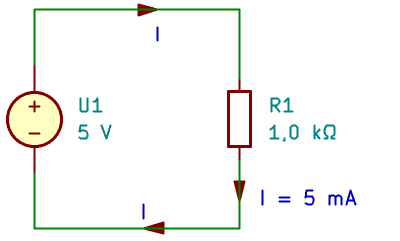
\includegraphics[width=8cm,height=\textheight,keepaspectratio]{_bilder/01-grunder-stromriktning.png}

\caption{\label{fig-grunder-stromriktning}Den konventionella strömmen
går ut ur källans pluspol och tillbaka till minuspolen genom resistorn.
Strömmen är lika stor överallt i kretsen i detta fall eftersom alla
komponenter är i serie.}

\end{figure}%

I en metall är de rörliga laddningsbärarna elektroner. Eftersom
elektroner är negativt laddade rör de sig i motsatt riktning mot den
definierade strömriktningen. Vid kretsanalys använder vi den definierade
strömriktningen. Vi behöver normalt inte bry oss om och följa
elektronernas rörelse.

\begin{tcolorbox}[enhanced jigsaw, arc=.35mm, bottomrule=.15mm, bottomtitle=1mm, breakable, colback=white, colbacktitle=quarto-callout-important-color!10!white, colframe=quarto-callout-important-color-frame, coltitle=black, left=2mm, leftrule=.75mm, opacityback=0, opacitybacktitle=0.6, rightrule=.15mm, title=\textcolor{quarto-callout-important-color}{\faExclamation}\hspace{0.5em}{Ström förbrukas inte}, titlerule=0mm, toprule=.15mm, toptitle=1mm]

När ström passerar en resistor omvandlas elektrisk energi till värme.
Strömmen förbrukas däremot inte. I ett stationärt tillstånd går lika
stor ström in i resistorns ena anslutning som ut ur den andra.

\end{tcolorbox}

\section{Elektrisk potential och
spänning}\label{sec-grunder-elektrisk-potential-och-spanning}

Potential och spänning har samma enhet, volt, men beskriver olika saker.

\textbf{Potential} anges för en punkt i förhållande till en vald
referens.

\textbf{Spänning} är \textbf{potentialskillnaden} mellan två punkter.

\begin{tcolorbox}[enhanced jigsaw, arc=.35mm, bottomrule=.15mm, bottomtitle=1mm, breakable, colback=white, colbacktitle=quarto-callout-tip-color!10!white, colframe=quarto-callout-tip-color-frame, coltitle=black, left=2mm, leftrule=.75mm, opacityback=0, opacitybacktitle=0.6, rightrule=.15mm, title=\textcolor{quarto-callout-tip-color}{\faLightbulb}\hspace{0.5em}{Potential och spänning -- jämför med höjd}, titlerule=0mm, toprule=.15mm, toptitle=1mm]

Elektrisk potential kan jämföras med \textbf{höjd över havet}. Havsnivån
är då vår valda referens, på samma sätt som jordpunkten tilldelas
potentialen \(0\,\mathrm{V}\) i en krets.

Spänning kan jämföras med \textbf{höjdskillnaden mellan två platser}.

Om plats A ligger 100 m över havet och plats B ligger 40 m över havet är
höjdskillnaden 60 m. På motsvarande sätt ger potentialerna
\(V_A = 100\,\mathrm{V}\) och \(V_B = 40\,\mathrm{V}\) spänningen

\[
U_{AB} = V_A - V_B = 60\,\mathrm{V}.
\]

Om vi väljer en annan referensnivå ändras platsernas angivna höjder, men
höjdskillnaden är densamma. På samma sätt ändrar ett byte av elektrisk
referenspunkt potentialernas värden, men inte spänningen mellan
punkterna.

\end{tcolorbox}

\subsection{Elektrisk potential}\label{sec-grunder-elektrisk-potential}

Elektrisk potential beskriver elektrisk potentiell energi per
laddningsenhet.

Vi väljer en \textbf{referenspunkt} och tilldelar den potentialen
\(0\,\mathrm{V}\). Därefter kan vi ange andra punkters potential i
förhållande till denna referens.

Om punkten A har potentialen

\[
V_A = 5\,\mathrm{V}
\]

betyder det att dess potential ligger \(5\,\mathrm{V}\) över den valda
referensens.

Potentialen kan också vara negativ. Om

\[
V_B = -2\,\mathrm{V}
\]

ligger punkten B:s potential \(2\,\mathrm{V}\) under referensens.

\subsection{Elektrisk spänning}\label{sec-grunder-elektrisk-spanning}

Spänningen från punkten A till punkten B definieras i denna bok som

\[
\boxed{U_{AB} = V_A - V_B}.
\]

Indexordningen är viktig. Om vi byter ordning får vi

\[
U_{BA} = V_B - V_A = -U_{AB}.
\]

Spänningen \(U_{AB}\) kan också markeras med plus vid A och minus vid B.
Markeringen anger hur spänningen är definierad.

Spänningens enhet är volt:

\[
[\mathrm{V}] = [\mathrm{J/C}].
\]

En potentialskillnad på \(1\,\mathrm{V}\) motsvarar alltså en skillnad i
elektrisk potentiell energi på \(1\,\mathrm{J}\) per coulomb laddning.

\begin{tcolorbox}[enhanced jigsaw, arc=.35mm, bottomrule=.15mm, bottomtitle=1mm, breakable, colback=white, colbacktitle=quarto-callout-note-color!10!white, colframe=quarto-callout-note-color-frame, coltitle=black, left=2mm, leftrule=.75mm, opacityback=0, opacitybacktitle=0.6, rightrule=.15mm, title={Exempel: spänning mellan två punkter}, titlerule=0mm, toprule=.15mm, toptitle=1mm]

Två punkter har potentialerna

\[
V_A = 5{,}0\,\mathrm{V},
\qquad
V_B = -2{,}0\,\mathrm{V}.
\]

\begin{figure}[H]

\centering{

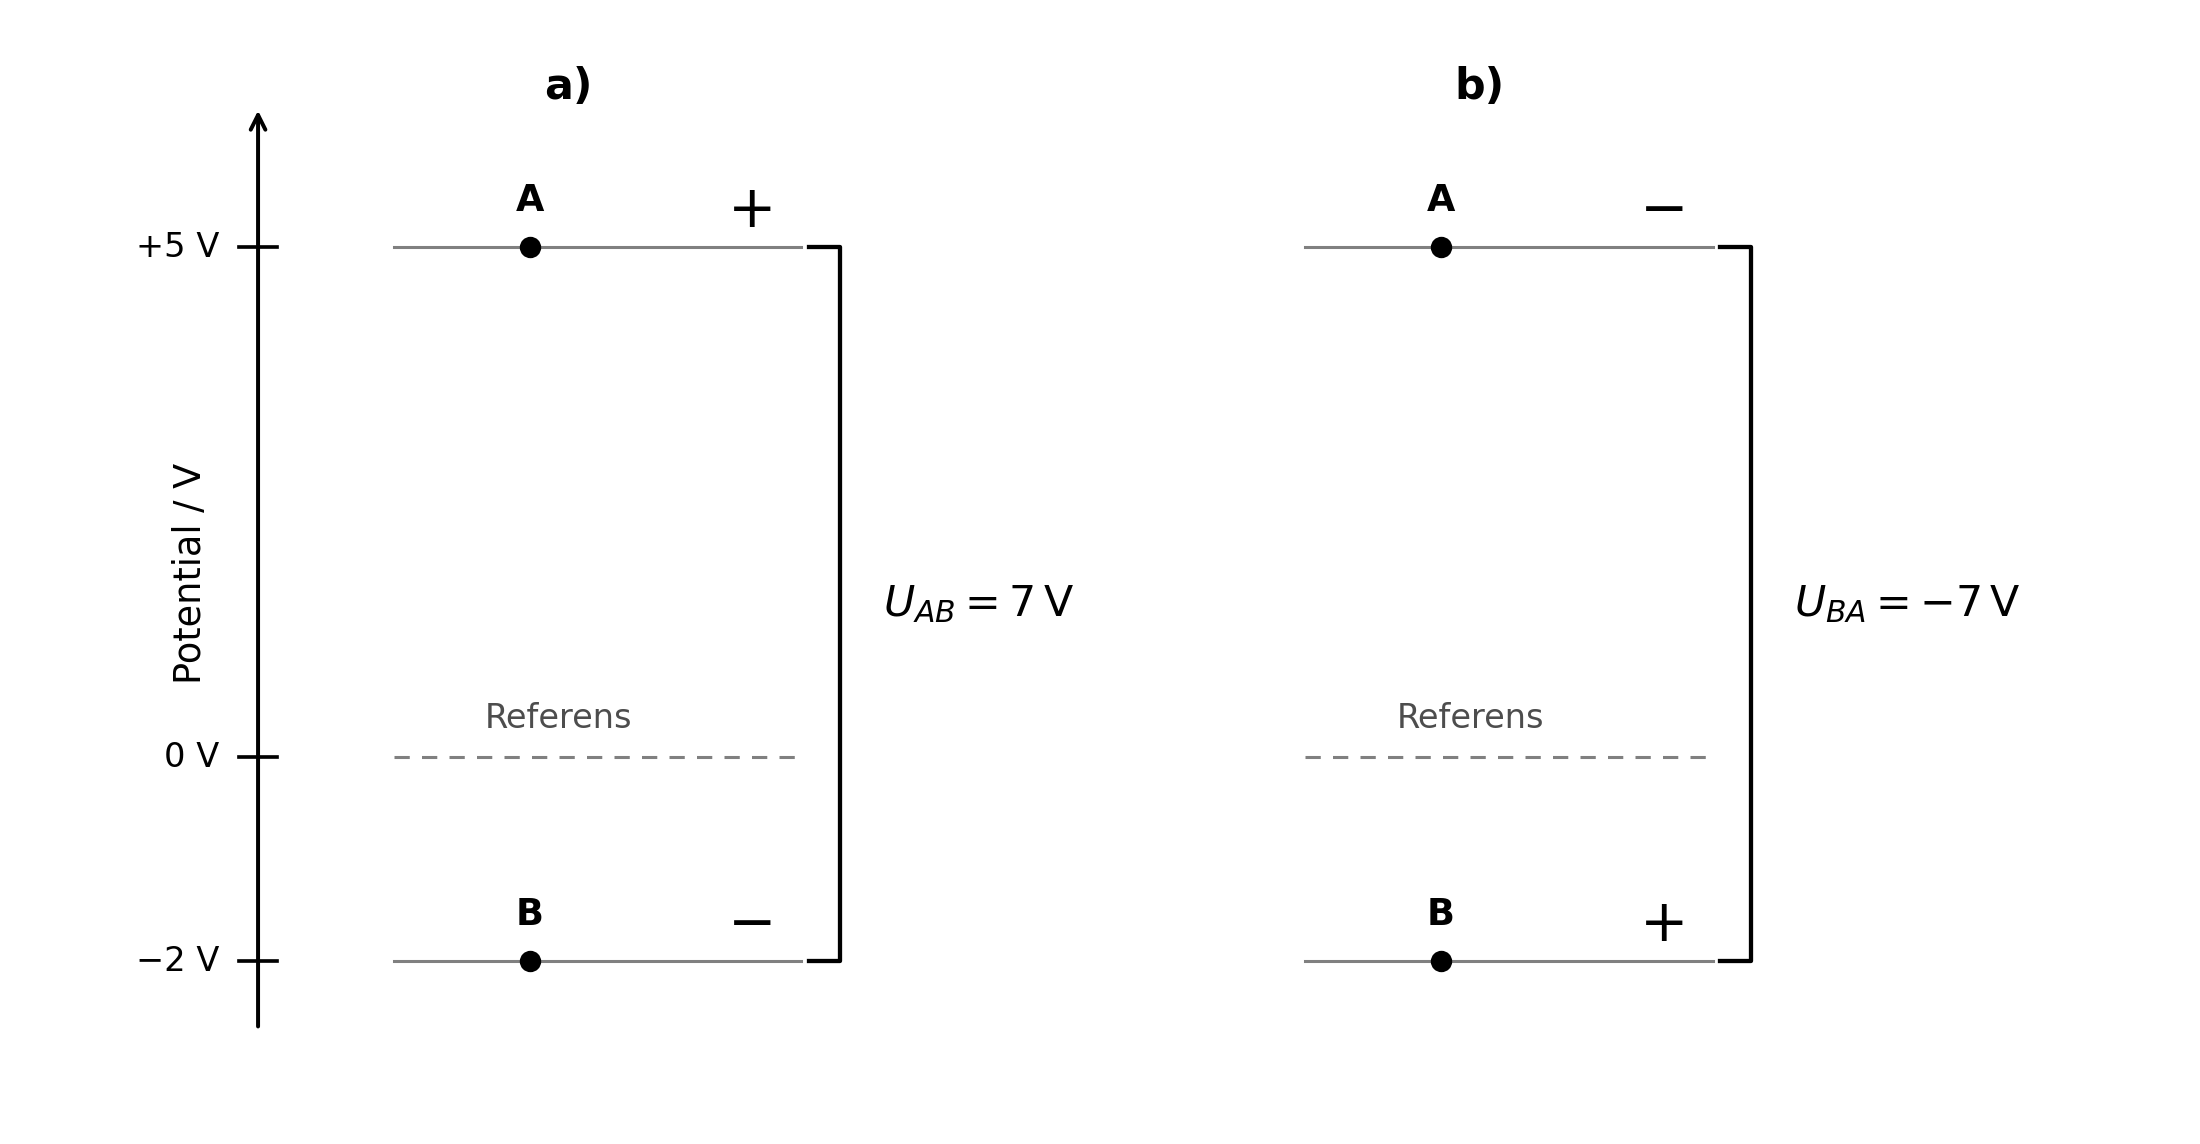
\includegraphics[width=14cm,height=\textheight,keepaspectratio]{_bilder/01-potential-och-spanning.png}

}

\caption{\label{fig-grunder-potential-spanning}Potentialerna anges
relativt referensen. Spänningens tecken beror på vilken polaritet som
definieras.}

\end{figure}%

\textbf{Lösning}

Spänningen från A till B blir

\[
U_{AB}
= V_A - V_B
= \bigl(5{,}0 - (-2{,}0)\bigr)\,\mathrm{V}
= 7{,}0\,\mathrm{V}.
\]

I motsatt riktning får vi

\[
U_{BA} = -7{,}0\,\mathrm{V}.
\]

\textbf{Svar:} \(U_{AB} = 7{,}0\,\mathrm{V}\) och
\(U_{BA} = -7{,}0\,\mathrm{V}\).

Det är samma potentialskillnad, men med två olika val av
\textbf{polaritet}.

\end{tcolorbox}

\section{Referenspunkt och
jord}\label{sec-grunder-referenspunkt-och-jord}

Referenspunkten i en krets kallas ofta \textbf{jord} och markeras med en
jordsymbol. Dess potential sätts till \(0\,\mathrm{V}\).

Valet av referens bestämmer vilka talvärden vi anger för kretsens
potentialer. Det förändrar däremot inte spänningarna mellan punkterna
eller strömmarna i kretsen.

\begin{tcolorbox}[enhanced jigsaw, arc=.35mm, bottomrule=.15mm, bottomtitle=1mm, breakable, colback=white, colbacktitle=quarto-callout-note-color!10!white, colframe=quarto-callout-note-color-frame, coltitle=black, left=2mm, leftrule=.75mm, opacityback=0, opacitybacktitle=0.6, rightrule=.15mm, title={Exempel: byte av referens}, titlerule=0mm, toprule=.15mm, toptitle=1mm]

Anta att vi först har följande potentialer (vänster kretsschema i
Figur~\ref{fig-grunder-byte-av-referens}):

\begin{longtable}[]{@{}ll@{}}
\caption{Potentialer med C som
referens.}\label{tbl-potentialer-c}\tabularnewline
\toprule\noalign{}
Punkt & Potential \\
\midrule\noalign{}
\endfirsthead
\toprule\noalign{}
Punkt & Potential \\
\midrule\noalign{}
\endhead
\bottomrule\noalign{}
\endlastfoot
A & \(12\,\mathrm{V}\) \\
B & \(5\,\mathrm{V}\) \\
C & \(0\,\mathrm{V}\) \\
\end{longtable}

Vi väljer nu B som ny referenspunkt (höger kretsschema i
Figur~\ref{fig-grunder-byte-av-referens}). Vi måste då subtrahera
\(5\,\mathrm{V}\) från samtliga potentialer:

\begin{longtable}[]{@{}ll@{}}
\caption{Potentialer med B som
referens.}\label{tbl-potentialer-b}\tabularnewline
\toprule\noalign{}
Punkt & Potential med B som referens \\
\midrule\noalign{}
\endfirsthead
\toprule\noalign{}
Punkt & Potential med B som referens \\
\midrule\noalign{}
\endhead
\bottomrule\noalign{}
\endlastfoot
A & \(7\,\mathrm{V}\) \\
B & \(0\,\mathrm{V}\) \\
C & \(-5\,\mathrm{V}\) \\
\end{longtable}

\begin{figure}[H]

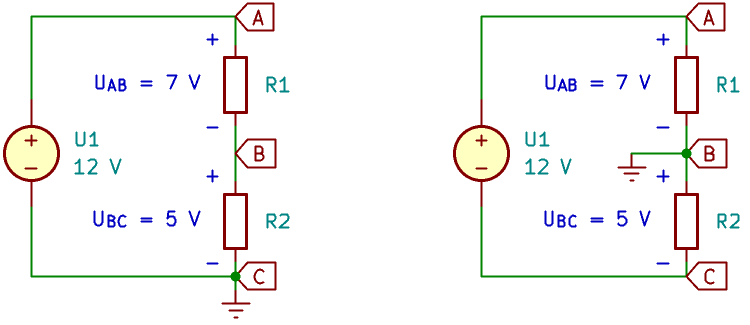
\includegraphics[width=15cm,height=\textheight,keepaspectratio]{_bilder/01-byte-av-referens.png}

\caption{\label{fig-grunder-byte-av-referens}Byte av referenspunkt
ändrar potentialernas talvärden. Kopplingen och spänningarna över
komponenterna är oförändrade. Det enda som ändrats är placeringen av
referenspunkten (jord). Detta gör att potentialerna i olika noder
förändras.}

\end{figure}%

Spänningen mellan A och C är fortfarande

\[
U_{AC} = V_A - V_C = \bigl(7 - (-5)\bigr)\,\mathrm{V} = 12\,\mathrm{V}.
\]

Vi har ändrat beskrivningen av kretsen och var referensen är placerad,
men inte själva kretsen.

\end{tcolorbox}

\begin{tcolorbox}[enhanced jigsaw, arc=.35mm, bottomrule=.15mm, bottomtitle=1mm, breakable, colback=white, colbacktitle=quarto-callout-important-color!10!white, colframe=quarto-callout-important-color-frame, coltitle=black, left=2mm, leftrule=.75mm, opacityback=0, opacitybacktitle=0.6, rightrule=.15mm, title=\textcolor{quarto-callout-important-color}{\faExclamation}\hspace{0.5em}{Jord är en referens -- ingen plats där ström försvinner}, titlerule=0mm, toprule=.15mm, toptitle=1mm]

En referenspunkt i ett kretsschema behöver inte vara ansluten till
marken eller till elnätets skyddsjord.

Signaljord, kretsens referens och skyddsjord kan ha olika funktioner.

En jordsymbol innebär inte att ström försvinner ur kretsen. Det är en
vanlig missuppfattning att all ström går till jord när en punkt markeras
med en jordsymbol.

I de stationära likströmskretsar vi behandlar här måste strömmen ha en
sluten väg tillbaka till källan. Ström kan flyta genom jordledningar,
men jordsymbolen i sig skapar ingen returväg.

\end{tcolorbox}

\textbf{Att välja en annan referens i en beräkning ska skiljas från att
fysiskt ansluta en jordad instrumentledning till kretsen.} En sådan
anslutning kan förändra kopplingen.

\section{Riktningar, polariteter och negativa
svar}\label{sec-grunder-riktningar-polariteter-och-negativa-svar}

Innan vi beräknar en ström behöver vi bestämma vilken riktning som ska
räknas som positiv. Den valda riktningen kallas
\textbf{referensriktning}. På motsvarande sätt behöver en spänning ha en
definierad polaritet.

Vi kan välja riktning även om vi ännu inte vet åt vilket håll strömmen
faktiskt flyter.

Om beräkningen ger

\[
I = -2{,}0\,\mathrm{mA}
\]

betyder det att strömmen är \(3\,\mathrm{mA}\) i motsatt riktning mot
den valda referensriktningen, se Figur~\ref{fig-grunder-negativ-strom}.

\begin{figure}

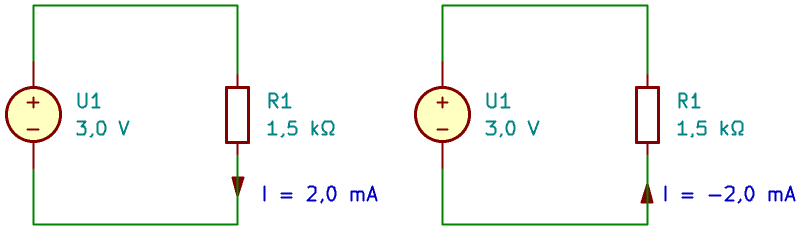
\includegraphics[width=16cm,height=\textheight,keepaspectratio]{_bilder/01-negativ-strom.png}

\caption{\label{fig-grunder-negativ-strom}Den verkliga strömmen i
kretsarna är medurs. Men samma verkliga ström kan beskrivas med ett
positivt eller negativt värde beroende på vald referensriktning.}

\end{figure}%

Ett negativt svar är alltså inte automatiskt ett fel.

\begin{tcolorbox}[enhanced jigsaw, arc=.35mm, bottomrule=.15mm, bottomtitle=1mm, breakable, colback=white, colbacktitle=quarto-callout-note-color!10!white, colframe=quarto-callout-note-color-frame, coltitle=black, left=2mm, leftrule=.75mm, opacityback=0, opacitybacktitle=0.6, rightrule=.15mm, title={Exempel: negativ spänning}, titlerule=0mm, toprule=.15mm, toptitle=1mm]

Vi definierar spänningen som

\[
U_{AB} = V_A - V_B.
\]

Om \(V_A = 2\,\mathrm{V}\) och \(V_B = 5\,\mathrm{V}\) blir

\[
U_{AB} = V_A - V_B
= (2 - 5)\,\mathrm{V}
= -3\,\mathrm{V}.
\]

Svaret betyder att B har högre potential än A.

\end{tcolorbox}

\section{Resistans och Ohms lag}\label{sec-ohms-lag}

En \textbf{resistor} är en komponent som begränsar strömmen i en krets.
\textbf{Resistans}, \(R\), är den elektriska storhet som beskriver
komponentens motstånd mot ström.

För en ideal linjär resistor gäller \textbf{Ohms lag}:

\[
\boxed{U = RI}.
\]

Här definieras strömmen som positiv in i resistorns anslutning märkt med
plus för spänningen \(U\).

Sambandet kan också skrivas

\[
\boxed{I = \frac{U}{R}}
\]

eller

\[
\boxed{R = \frac{U}{I}}.
\]

Resistansens enhet är ohm:

\[
[\Omega] = [\mathrm{V/A}].
\]

För en given spänning ger en större resistans en mindre ström.

\subsection{Linjär resistor}\label{sec-grunder-linjar-resistor}

Att resistorn är \textbf{linjär} innebär att strömmen är proportionell
mot spänningen. Om spänningen fördubblas fördubblas strömmen.

I ett diagram (Figur~\ref{fig-grunder-ohms-lag}) med spänning på den
horisontella axeln och ström på den vertikala blir sambandet en rät
linje genom origo. Linjens lutning är \(1/R\).

\begin{figure}

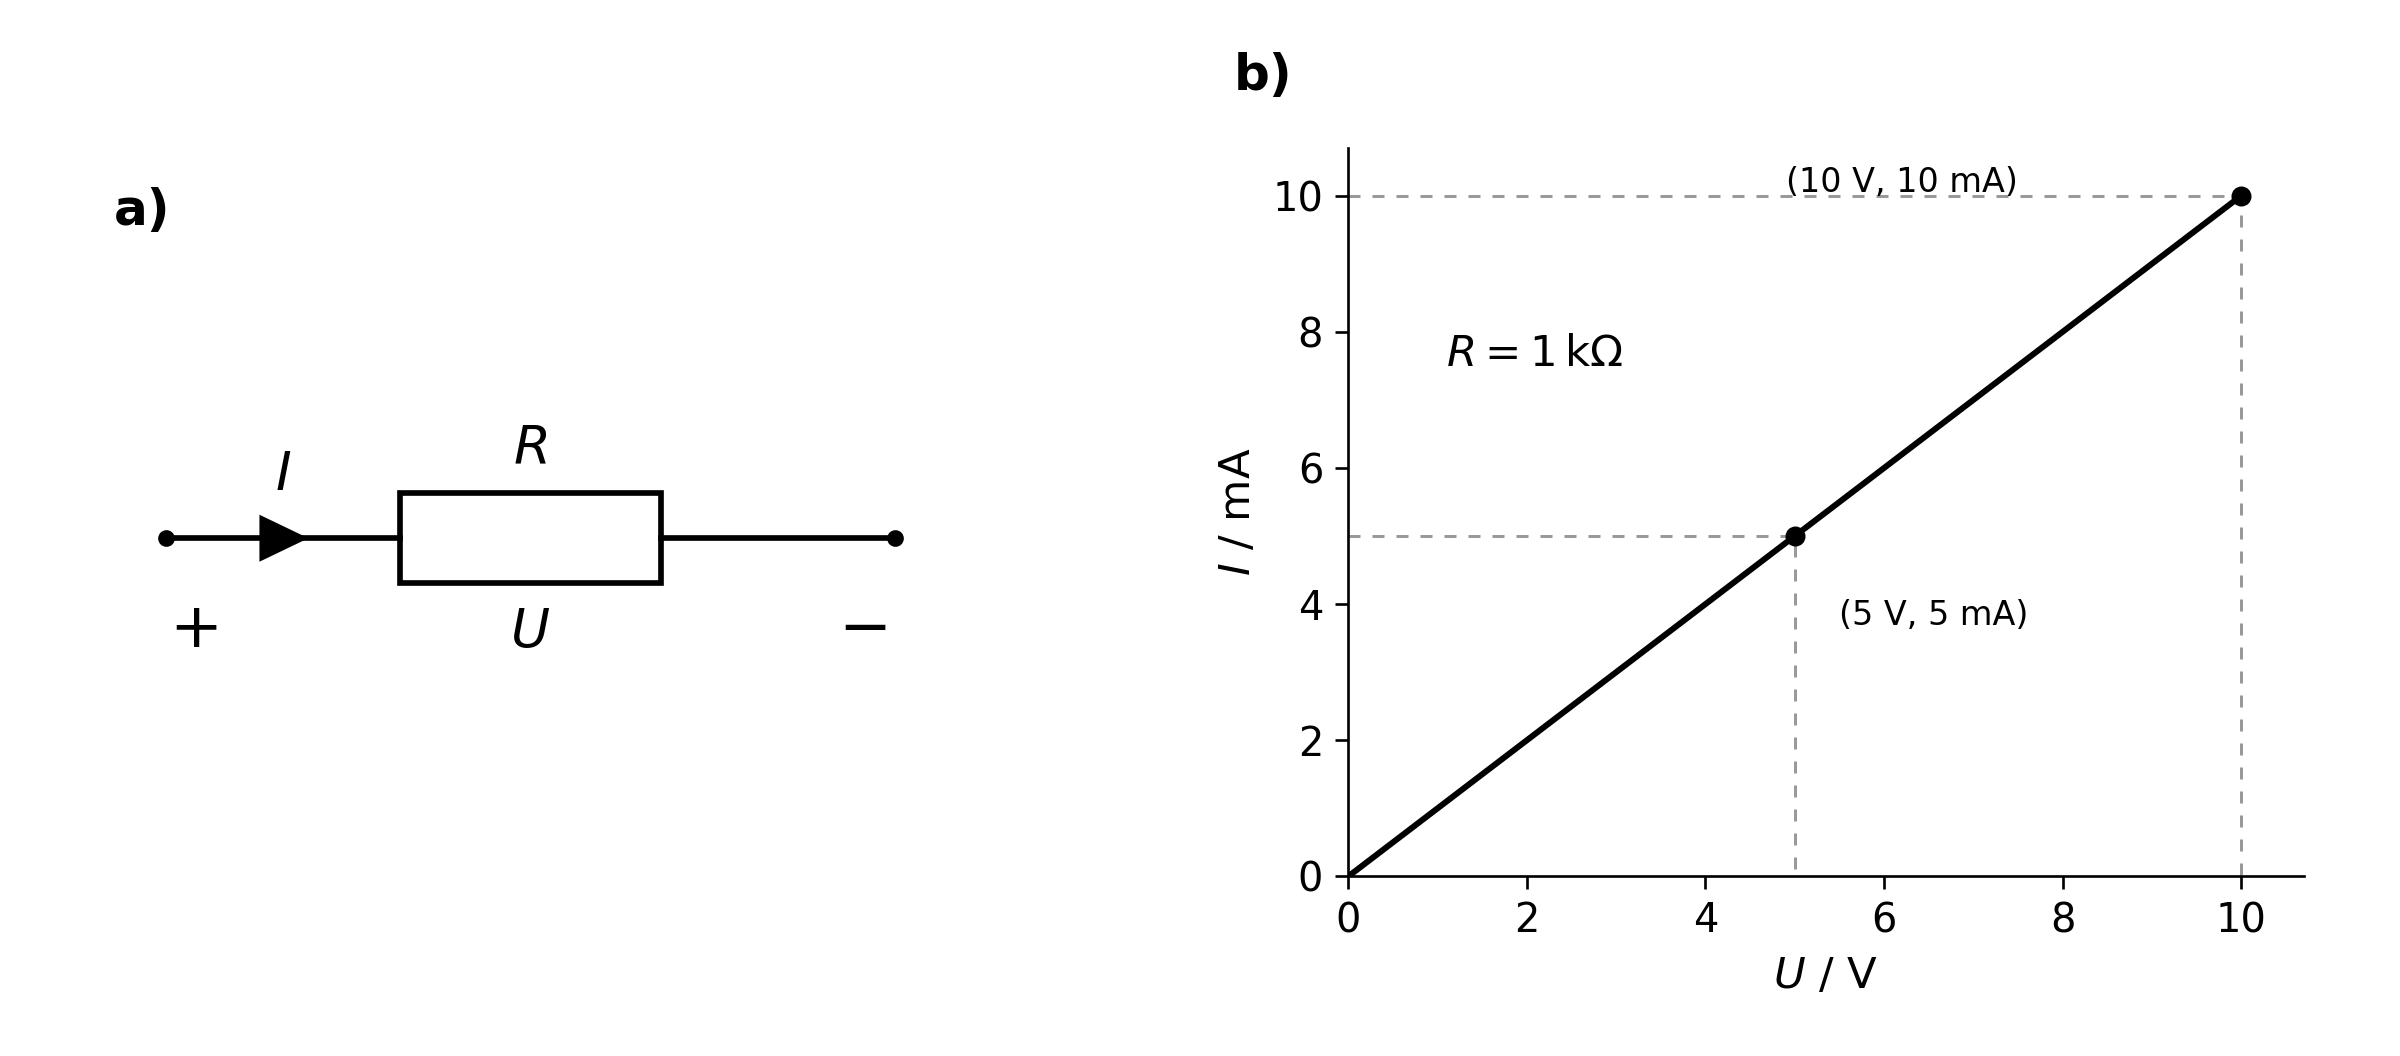
\includegraphics[width=14cm,height=\textheight,keepaspectratio]{_bilder/01-ohms-lag.png}

\caption{\label{fig-grunder-ohms-lag}Resistorns spänning och
strömriktning samt det linjära sambandet mellan ström och spänning för R
= 1 kΩ.}

\end{figure}%

\begin{tcolorbox}[enhanced jigsaw, arc=.35mm, bottomrule=.15mm, bottomtitle=1mm, breakable, colback=white, colbacktitle=quarto-callout-important-color!10!white, colframe=quarto-callout-important-color-frame, coltitle=black, left=2mm, leftrule=.75mm, opacityback=0, opacitybacktitle=0.6, rightrule=.15mm, title=\textcolor{quarto-callout-important-color}{\faExclamation}\hspace{0.5em}{Ohms lag är en idealiserad modell}, titlerule=0mm, toprule=.15mm, toptitle=1mm]

Sambandet \(U = RI\) med konstant resistans beskriver en ideal linjär
resistor. Vi använder det som en \textbf{modell} för en verklig
resistor, som följer modellen ungefärligt inom ett begränsat
arbetsområde.

Resistansen påverkas bland annat av temperaturen. När strömmen värmer
upp resistorn kan resistansen förändras, vilket gör att strömmen inte
längre är exakt proportionell mot spänningen.

Modellen med konstant resistans är ändå ofta tillräckligt noggrann för
våra beräkningar. Vi behöver bedöma om den är rimlig för komponentens
arbetsförhållanden och den noggrannhet vi behöver.

\end{tcolorbox}

\begin{tcolorbox}[enhanced jigsaw, arc=.35mm, bottomrule=.15mm, bottomtitle=1mm, breakable, colback=white, colbacktitle=quarto-callout-note-color!10!white, colframe=quarto-callout-note-color-frame, coltitle=black, left=2mm, leftrule=.75mm, opacityback=0, opacitybacktitle=0.6, rightrule=.15mm, title={Exempel: ström genom en resistor}, titlerule=0mm, toprule=.15mm, toptitle=1mm]

En resistor med resistansen \(2{,}2\,\mathrm{k}\Omega\) ansluts till
spänningen \(5{,}0\,\mathrm{V}\).

Strömmen blir

\[
I = \frac{U}{R}
= \frac{5{,}0}{2200}\,\mathrm{A}
\approx 2{,}3\,\mathrm{mA}.
\]

\textbf{Rimlighetskontroll:} Vid \(2{,}2\,\mathrm{V}\) skulle strömmen
vara \(1\,\mathrm{mA}\). Vid \(5{,}0\,\mathrm{V}\) bör den därför vara
lite mer än dubbelt så stor.

\end{tcolorbox}

\begin{tcolorbox}[enhanced jigsaw, arc=.35mm, bottomrule=.15mm, bottomtitle=1mm, breakable, colback=white, colbacktitle=quarto-callout-note-color!10!white, colframe=quarto-callout-note-color-frame, coltitle=black, left=2mm, leftrule=.75mm, opacityback=0, opacitybacktitle=0.6, rightrule=.15mm, title={Exempel: bestäm resistansen}, titlerule=0mm, toprule=.15mm, toptitle=1mm]

Spänningen över en resistor mäts till \(3{,}6\,\mathrm{V}\) och strömmen
genom den till \(12\,\mathrm{mA}\).

Resistansen blir

\[
R = \frac{U}{I}
= \frac{3{,}6}{0{,}012}\,\Omega
= 300\,\Omega.
\]

\end{tcolorbox}

\section{Konduktans}\label{sec-grunder-konduktans}

\textbf{Konduktans} beskriver hur lätt en komponent leder ström.
Konduktansen betecknas \(G\) och definieras som resistansens invers:

\[
\boxed{G = \frac{1}{R}}.
\]

Enheten är siemens:

\[
[\mathrm{S}] = [\Omega^{-1}].
\]

Ohms lag kan därför även skrivas

\[
\boxed{I = GU}.
\]

Hög resistans innebär låg konduktans. Låg resistans innebär hög
konduktans.

\begin{tcolorbox}[enhanced jigsaw, arc=.35mm, bottomrule=.15mm, bottomtitle=1mm, breakable, colback=white, colbacktitle=quarto-callout-note-color!10!white, colframe=quarto-callout-note-color-frame, coltitle=black, left=2mm, leftrule=.75mm, opacityback=0, opacitybacktitle=0.6, rightrule=.15mm, title={Exempel: från resistans till konduktans}, titlerule=0mm, toprule=.15mm, toptitle=1mm]

En resistor har resistansen
\(R = 2{,}0\,\mathrm{k}\Omega = 2000\,\Omega\).

Dess konduktans är

\[
G = \frac{1}{R}
= \frac{1}{2000}\,\mathrm{S}
= 0{,}00050\,\mathrm{S}
= 0{,}50\,\mathrm{mS}.
\]

Konduktans blir särskilt användbar när vi senare arbetar med
parallellkopplingar.

\end{tcolorbox}

\section{Resistans i en ledare}\label{sec-grunder-resistans-i-en-ledare}

Även ledningar har resistans. \textbf{Resistivitet} är en
materialegenskap som beskriver hur starkt materialet motverkar elektrisk
ström. Ledarens resistans beror dessutom på dess längd och
\textbf{tvärsnittsarea}. För en homogen ledare med konstant
tvärsnittsarea (se exempelt med ledare med cirkulärt tvärsnitt i
Figur~\ref{fig-grunder-ledarens-resistans}) gäller

\[
\boxed{R = \rho\frac{l}{A}},
\]

där

\begin{itemize}
\item
  \(\rho\) är materialets resistivitet,
\item
  \(l\) är ledarens längd,
\item
  \(A\) är ledarens tvärsnittsarea.
\end{itemize}

\begin{figure}

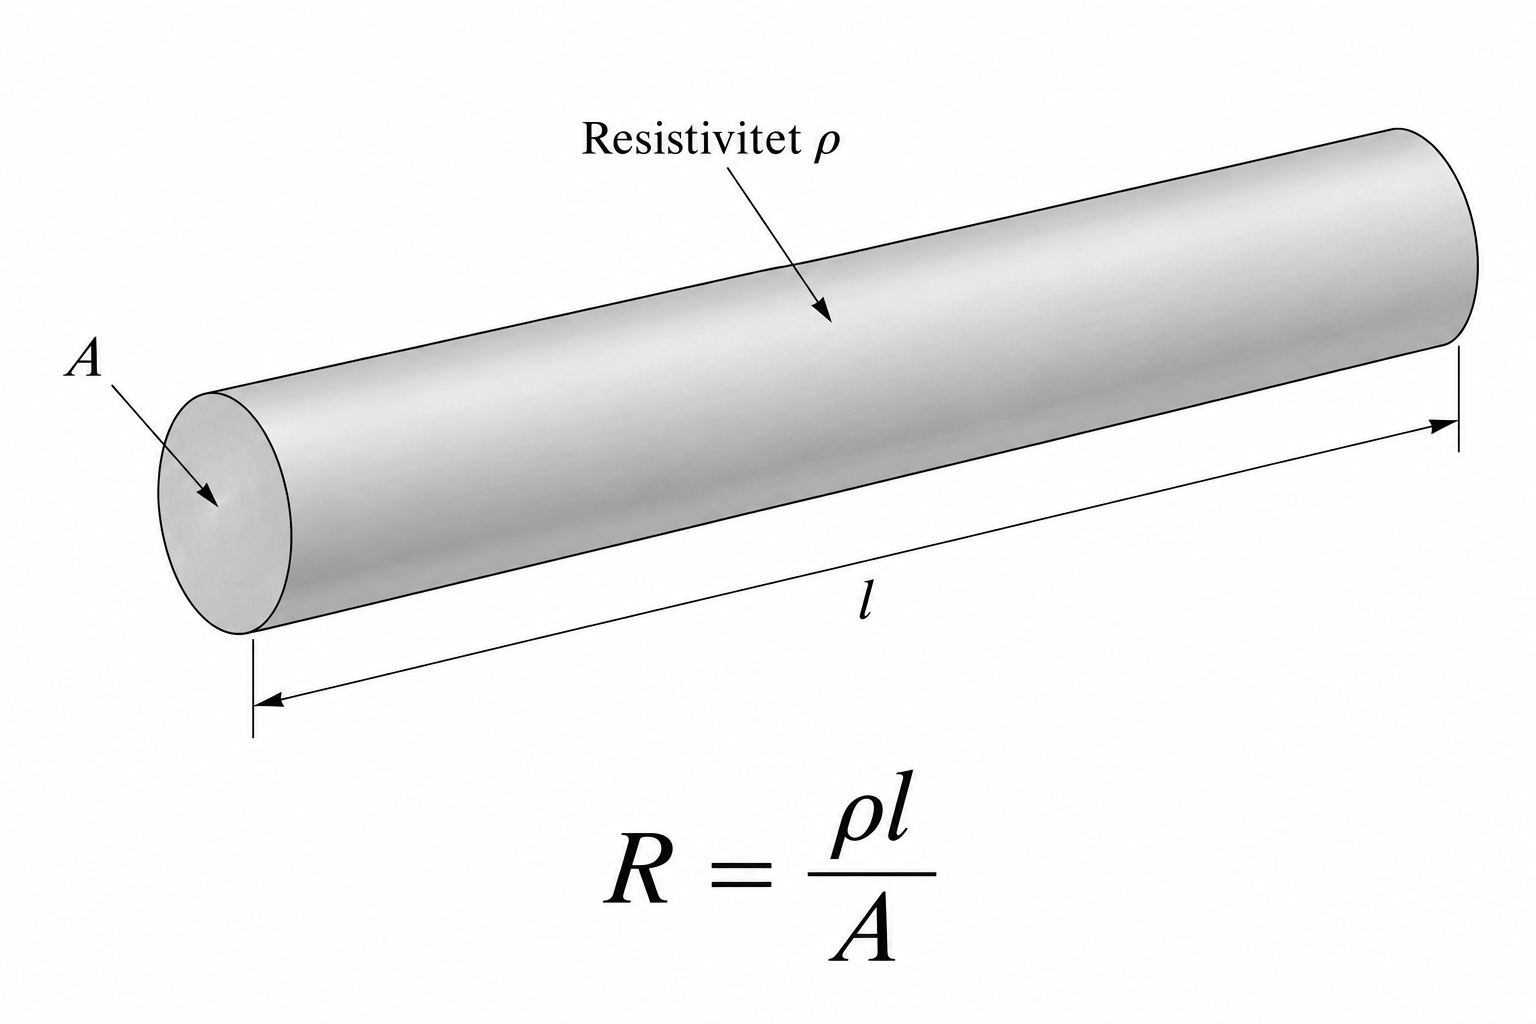
\includegraphics[width=6cm,height=\textheight,keepaspectratio]{_bilder/01-resistans-ledare.png}

\caption{\label{fig-grunder-ledarens-resistans}Ledningens resistans
beror på materialets resistivitet, ledarens längd och dess
tvärsnittsarea.}

\end{figure}%

Om \(\rho\) anges i \(\Omega\,\mathrm{m}\) ska längden anges i meter och
arean i kvadratmeter.

Sambandet visar att:

\begin{itemize}
\item
  en längre ledare har högre resistans,
\item
  en grövre ledare har lägre resistans,
\item
  material med högre resistivitet ger högre resistans.
\end{itemize}

Resistiviteten beror bland annat på material och temperatur.

\begin{tcolorbox}[enhanced jigsaw, arc=.35mm, bottomrule=.15mm, bottomtitle=1mm, breakable, colback=white, colbacktitle=quarto-callout-note-color!10!white, colframe=quarto-callout-note-color-frame, coltitle=black, left=2mm, leftrule=.75mm, opacityback=0, opacitybacktitle=0.6, rightrule=.15mm, title={Exempel: resistans i en kopparledning}, titlerule=0mm, toprule=.15mm, toptitle=1mm]

Använd det avrundade värdet

\[
\rho = 0{,}0175\,\Omega\,\mathrm{mm^2/m}
\]

för koppar vid ungefär rumstemperatur.

En ledare är \(2{,}0\,\mathrm{m}\) lång och har arean
\(0{,}50\,\mathrm{mm^2}\). Dess resistans blir

\[
R = \rho\frac{l}{A}
= \left(0{,}0175 \cdot \frac{2{,}0}{0{,}50}\right)\,\Omega
= 0{,}070\,\Omega.
\]

Vid strömmen \(1{,}0\,\mathrm{A}\) blir \textbf{spänningsfallet}

\[
U = RI
= (0{,}070 \cdot 1{,}0)\,\mathrm{V}
= 0{,}070\,\mathrm{V}.
\]

Om strömmen går till en last genom en ledare och tillbaka genom en lika
lång ledare blir den sammanlagda ledningsresistansen dubbelt så stor.

\end{tcolorbox}

\section{Ideala källor}\label{sec-grunder-ideala-kallor}

\subsection{Ideal
spänningskälla}\label{sec-grunder-ideal-spanningskalla}

En \textbf{ideal spänningskälla} håller en bestämd spänning mellan sina
anslutningar, oberoende av vilken ström som tas ut.

Strömmen bestäms av den anslutna kretsen, som vi kallar \textbf{lasten}.

Om lasten är en resistor gäller

\[
I = \frac{U}{R}.
\]

En mindre lastresistans ger alltså större ström, medan källans spänning
är oförändrad.

Vid \textbf{tomgång}, när ingen last är ansluten, är strömmen noll.

Spänningen mellan källans anslutningar finns ändå kvar.

\begin{tcolorbox}[enhanced jigsaw, arc=.35mm, bottomrule=.15mm, bottomtitle=1mm, breakable, colback=white, colbacktitle=quarto-callout-note-color!10!white, colframe=quarto-callout-note-color-frame, coltitle=black, left=2mm, leftrule=.75mm, opacityback=0, opacitybacktitle=0.6, rightrule=.15mm, title={Exempel: ideal spänningskälla}, titlerule=0mm, toprule=.15mm, toptitle=1mm]

En ideal spänningskälla håller spänningen \(U_1 = 10\,\mathrm{V}\)
(Figur~\ref{fig-grunder-ideal-spanningskalla}).

\begin{figure}[H]

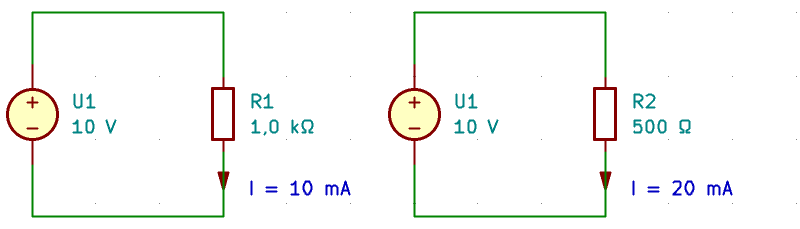
\includegraphics[width=16cm,height=\textheight,keepaspectratio]{_bilder/01-ideal-spanningskalla.png}

\caption{\label{fig-grunder-ideal-spanningskalla}En ideal spänningskälla
håller spänningen konstant. Strömmen ändras när lastresistansen ändras.}

\end{figure}%

Med lastresistansen \(R_1 = 1000\,\Omega\) blir strömmen

\[
I = \frac{U_1}{R_1}
= \frac{10}{1000}\,\mathrm{A}
= 10\,\mathrm{mA}.
\]

Om resistansen minskas till \(500\,\Omega\) blir strömmen

\[
I = \frac{U_1}{R_2}
= \frac{10}{500}\,\mathrm{A}
= 20\,\mathrm{mA}.
\]

Strömmen fördubblas, men spänningen är fortfarande \(10\,\mathrm{V}\).

\end{tcolorbox}

\subsection{Ideal strömkälla}\label{sec-grunder-ideal-stromkalla}

En \textbf{ideal strömkälla} håller en bestämd ström genom den anslutna
kretsen, oberoende av vilken spänning som behövs.

Spänningen bestäms av lasten. Om lasten är en resistor gäller

\[
U = RI.
\]

En större lastresistans kräver alltså högre spänning, medan strömmen är
oförändrad.

Vid \textbf{kortslutning} är spänningen över den ideala förbindelsen
noll.

Strömkällan ger fortfarande sin bestämda ström.

\begin{tcolorbox}[enhanced jigsaw, arc=.35mm, bottomrule=.15mm, bottomtitle=1mm, breakable, colback=white, colbacktitle=quarto-callout-note-color!10!white, colframe=quarto-callout-note-color-frame, coltitle=black, left=2mm, leftrule=.75mm, opacityback=0, opacitybacktitle=0.6, rightrule=.15mm, title={Exempel: ideal strömkälla}, titlerule=0mm, toprule=.15mm, toptitle=1mm]

En ideal strömkälla håller strömmen \(I_1 = 10\,\mathrm{mA}\)
(Figur~\ref{fig-grunder-ideal-stromkalla}).

\begin{figure}[H]

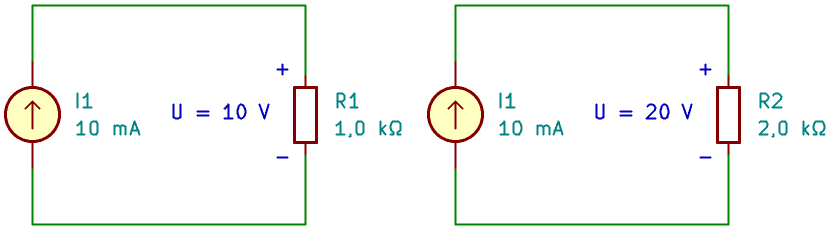
\includegraphics[width=16cm,height=\textheight,keepaspectratio]{_bilder/01-ideal-stromkalla.png}

\caption{\label{fig-grunder-ideal-stromkalla}En ideal strömkälla håller
strömmen konstant. Spänningen ändras när lastresistansen ändras.}

\end{figure}%

\[
U = R_{1}I_{1}
= (1000 \cdot 0{,}010)\,\mathrm{V}
= 10\,\mathrm{V}.
\]

Om resistansen ökas till \(2000\,\Omega\) blir spänningen

\[
U = R_{2}I_{1}
= (2000 \cdot 0{,}010)\,\mathrm{V}
= 20\,\mathrm{V}.
\]

Spänningen fördubblas, men strömmen är fortfarande \(10\,\mathrm{mA}\).

\end{tcolorbox}

\begin{tcolorbox}[enhanced jigsaw, arc=.35mm, bottomrule=.15mm, bottomtitle=1mm, breakable, colback=white, colbacktitle=quarto-callout-important-color!10!white, colframe=quarto-callout-important-color-frame, coltitle=black, left=2mm, leftrule=.75mm, opacityback=0, opacitybacktitle=0.6, rightrule=.15mm, title=\textcolor{quarto-callout-important-color}{\faExclamation}\hspace{0.5em}{Ideala källor är modeller}, titlerule=0mm, toprule=.15mm, toptitle=1mm]

En ideal spänningskälla kan enligt modellen ge hur stor ström som helst.
En ideal strömkälla kan enligt modellen ge hur hög spänning som helst.
Verkliga källor har däremot begränsningar i ström, spänning och effekt.

Modellerna har också gränsfall där de inte ger något ändligt resultat:
en ideal spänningskälla med spänning skild från noll kan inte
kortslutas, och en ideal strömkälla med ström skild från noll kan inte
lämnas med öppen krets.

Vi använder idealmodellerna när verkliga källors begränsningar inte
påverkar kretsens funktion.

\end{tcolorbox}

\section{Kirchhoffs strömlag}\label{sec-grunder-kirchhoffs-stromlag}

En \textbf{nod} är en elektriskt sammanhängande del av kretsen. Alla
punkter som är förbundna med ideala ledningar utan någon komponent
mellan sig tillhör samma nod och har samma potential.

\textbf{Kirchhoffs strömlag} beskriver hur strömmarna förhåller sig vid
en nod:

\begin{quote}
Summan av strömmarna in i en nod är lika med summan av strömmarna ut ur
noden.
\end{quote}

Vi kan också uttrycka lagen med en teckenkonvention. Om strömmar in i
noden räknas som positiva och strömmar ut som negativa gäller

\[
\boxed{\sum_k I_k = 0}.
\]

Lagen bygger på att laddning bevaras. I den idealiserade noden ansamlas
ingen laddning.

\begin{tcolorbox}[enhanced jigsaw, arc=.35mm, bottomrule=.15mm, bottomtitle=1mm, breakable, colback=white, colbacktitle=quarto-callout-note-color!10!white, colframe=quarto-callout-note-color-frame, coltitle=black, left=2mm, leftrule=.75mm, opacityback=0, opacitybacktitle=0.6, rightrule=.15mm, title={Exempel: ström i en förgrening}, titlerule=0mm, toprule=.15mm, toptitle=1mm]

\begin{figure}[H]

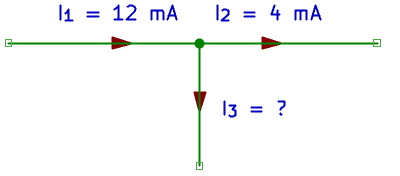
\includegraphics[width=8cm,height=\textheight,keepaspectratio]{_bilder/01-stromforgrening.png}

\caption{\label{fig-grunder-stromforgrening}Strömmarnas
referensriktningar vid en nod. Summan av strömmarna in är lika med
summan ut.}

\end{figure}%

Se urklippet i kretsschemat i Figur~\ref{fig-grunder-stromforgrening}.
Strömmen \(I_1 = 12\,\mathrm{mA}\) går in i en nod. Två strömmar,
\(I_2\) och \(I_3\), går ut.

Om \(I_2 = 4\,\mathrm{mA}\) ger strömlagen

\[
I_1 - I_2 - I_3 = 0.
\]

Vi löser ut \(I_3\):

\[
I_3 = I_1 - I_2
= (12 - 4)\,\mathrm{mA}
= 8\,\mathrm{mA}.
\]

\textbf{Kontroll:} Totalt går \(12\,\mathrm{mA}\) in och
\((4+8)\,\mathrm{mA}=12\,\mathrm{mA}\) ut.

\end{tcolorbox}

\begin{tcolorbox}[enhanced jigsaw, arc=.35mm, bottomrule=.15mm, bottomtitle=1mm, breakable, colback=white, colbacktitle=quarto-callout-note-color!10!white, colframe=quarto-callout-note-color-frame, coltitle=black, left=2mm, leftrule=.75mm, opacityback=0, opacitybacktitle=0.6, rightrule=.15mm, title={Exempel: en antagen riktning visar sig vara fel}, titlerule=0mm, toprule=.15mm, toptitle=1mm]

Anta i stället att \(I_1 = 5\,\mathrm{mA}\) och
\(I_2 = 8\,\mathrm{mA}\), med samma definierade riktningar
(Figur~\ref{fig-grunder-stromforgrening-negativ}).

\begin{figure}[H]

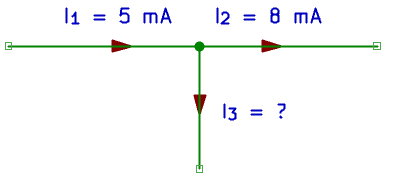
\includegraphics[width=8cm,height=\textheight,keepaspectratio]{_bilder/01-stromforgrening-negativ-strom.png}

\caption{\label{fig-grunder-stromforgrening-negativ}Strömmarnas
referensriktningar vid en nod. Om någon referensriktning går motsatt
riktning den fysiska strömmen ger detta negativt tecken.}

\end{figure}%

Då blir

\[
I_3 = I_1 - I_2 = (5 - 8)\,\mathrm{mA} = -3\,\mathrm{mA}.
\]

Strömmen \(I_3\) går alltså i verkligheten in i noden. Då går totalt
\((5+3)\,\mathrm{mA}=8\,\mathrm{mA}\) in och \(8\,\mathrm{mA}\) ut.

\end{tcolorbox}

\section{Kirchhoffs
spänningslag}\label{sec-grunder-kirchhoffs-spanningslag}

\textbf{Kirchhoffs spänningslag} beskriver spänningarna längs en sluten
väg i en krets:

\begin{quote}
Den algebraiska summan av spänningsändringarna längs en sluten väg är
noll.
\end{quote}

Vi skriver detta som

\[
\boxed{\sum_k \Delta V_k = 0}.
\]

Välj först en riktning att följa runt kretsen. När du passerar en
komponent gäller:

\begin{itemize}
\item
  från minus till plus: en positiv potentialändring,
\item
  från plus till minus: en negativ potentialändring.
\end{itemize}

När du återkommer till startpunkten måste potentialen vara densamma som
när du började.

\begin{tcolorbox}[enhanced jigsaw, arc=.35mm, bottomrule=.15mm, bottomtitle=1mm, breakable, colback=white, colbacktitle=quarto-callout-note-color!10!white, colframe=quarto-callout-note-color-frame, coltitle=black, left=2mm, leftrule=.75mm, opacityback=0, opacitybacktitle=0.6, rightrule=.15mm, title={Exempel: källa och två resistorer}, titlerule=0mm, toprule=.15mm, toptitle=1mm]

En sluten krets består av en ideal spänningskälla på \(12\,\mathrm{V}\)
och två resistorer som är kopplade efter varandra
(Figur~\ref{fig-grunder-spanningslagen}).

\begin{figure}[H]

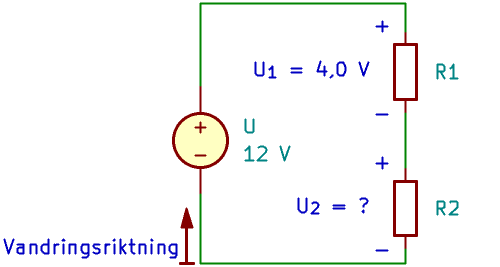
\includegraphics[width=10cm,height=\textheight,keepaspectratio]{_bilder/01-spanningslagen.png}

\caption{\label{fig-grunder-spanningslagen}Ett varv runt slingan ger
spänningshöjningen \(U\) och spänningsfallen \(U_1\) och \(U_2\).
Vandringen slutar vid samma potential som den började.}

\end{figure}%

Vi följer kretsen från källans minuspol genom källan till dess pluspol
och därefter genom de två resistorerna tillbaka till startpunkten.

Om källspänningen betecknas \(U\) och spänningsfallen över resistorerna
är \(U_1\) och \(U_2\) får vi

\[
U - U_1 - U_2 = 0.
\]

Om \(U_1 = 4{,}0\,\mathrm{V}\) blir

\[
U_2 = U - U_1 = (12 - 4{,}0)\,\mathrm{V} = 8{,}0\,\mathrm{V}.
\]

Spänningsfallen över resistorerna summeras alltså till källans spänning.

\end{tcolorbox}

\begin{tcolorbox}[enhanced jigsaw, arc=.35mm, bottomrule=.15mm, bottomtitle=1mm, breakable, colback=white, colbacktitle=quarto-callout-important-color!10!white, colframe=quarto-callout-important-color-frame, coltitle=black, left=2mm, leftrule=.75mm, opacityback=0, opacitybacktitle=0.6, rightrule=.15mm, title=\textcolor{quarto-callout-important-color}{\faExclamation}\hspace{0.5em}{Lagarna används i en kretsmodell}, titlerule=0mm, toprule=.15mm, toptitle=1mm]

Kirchhoffs lagar används genom hela boken. Här arbetar vi med kretsar
där ledningarnas egenskaper kan försummas och komponenterna kan
beskrivas var för sig.

Om ett tidsvarierande magnetiskt flöde genom kretsen ger en inducerad
spänning måste även denna tas med i modellen.

\end{tcolorbox}

\begin{tcolorbox}[enhanced jigsaw, arc=.35mm, bottomrule=.15mm, bottomtitle=1mm, breakable, colback=white, colbacktitle=quarto-callout-note-color!10!white, colframe=quarto-callout-note-color-frame, coltitle=black, left=2mm, leftrule=.75mm, opacityback=0, opacitybacktitle=0.6, rightrule=.15mm, title={Exempel: en enkel, sammanhängande kretsberäkning}, titlerule=0mm, toprule=.15mm, toptitle=1mm]

En ideal spänningskälla på \(9{,}0\,\mathrm{V}\) är ansluten till en
resistor med resistansen \(1{,}5\,\mathrm{k}\Omega\). Resistorns andra
anslutning är kopplad tillbaka till källans minuspol
(Figur~\ref{fig-grunder-kretsberakning} ).

Vi kallar källans pluspol A och minuspol B.

\textbf{Välj referens och riktningar}

Vi väljer B som referens (jord):

\begin{figure}[H]

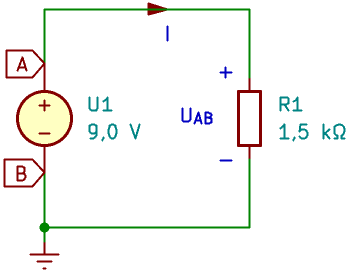
\includegraphics[width=7cm,height=\textheight,keepaspectratio]{_bilder/01-kretsberakning.png}

\caption{\label{fig-grunder-kretsberakning}Enkel krets med ideal
spänningskälla och resistor. Kretsens noder, referenspunkt,
strömriktning och spänningspolaritet definieras innan beräkningen
börjar.}

\end{figure}%

\[
V_B = 0\,\mathrm{V}.
\]

Källan bestämmer då potentialen i A:

\[
V_A = 9{,}0\,\mathrm{V}.
\]

Strömmen \(I\) definieras från A genom resistorn till B.

\textbf{Bestäm spänningen över resistorn}

Spänningen definieras med plus vid A och minus vid B:

\[
U_{AB}
= V_A - V_B
= (9{,}0 - 0)\,\mathrm{V}
= 9{,}0\,\mathrm{V}.
\]

\textbf{Beräkna strömmen}

Ohms lag ger

\[
I
= \frac{U_{AB}}{R}
= \frac{9{,}0}{1500}\,\mathrm{A}
= 6{,}0\,\mathrm{mA}.
\]

Det positiva svaret betyder att strömmen går i den valda riktningen.

\textbf{Kontrollera resultatet}

Kirchhoffs spänningslag ger

\[
U_{AB} - RI
= (9{,}0 - 1500 \cdot 0{,}0060)\,\mathrm{V}
= 0\,\mathrm{V}.
\]

Strömmen är också lika stor överallt i kretsens enda strömväg.

Om vi väljer A som referens i stället får vi

\[
V_A = 0\,\mathrm{V},
\qquad
V_B = -9{,}0\,\mathrm{V}.
\]

Spänningen över resistorn är fortfarande \(9{,}0\,\mathrm{V}\) och
strömmen fortfarande \(6{,}0\,\mathrm{mA}\).

\end{tcolorbox}

\section{En arbetsgång för
kretsberäkningar}\label{sec-grunder-en-arbetsgang-for-kretsberakningar}

En tydlig arbetsgång minskar risken för fel och gör lösningen lättare
att följa.

\begin{enumerate}
\def\labelenumi{\arabic{enumi}.}
\item
  \textbf{Identifiera vad som söks.} Är det en ström, en spänning, en
  potential eller en resistans?
\item
  \textbf{Markera givna värden.} Skriv in värden och enheter i schemat.
\item
  \textbf{Välj referens och riktningar.} Markera jordpunkt, strömpilar
  och spänningspolariteter.
\item
  \textbf{Skriv sambanden med symboler.} Använd exempelvis Ohms lag och
  Kirchhoffs lagar.
\item
  \textbf{Lös ut den sökta storheten.}
\item
  \textbf{Sätt in talvärden och ange enheten efter det numeriska
  uttrycket.} Kontrollera att valda enheter och prefix ger rätt
  resultatenhet.
\item
  \textbf{Kontrollera och tolka resultatet.}
\end{enumerate}

Behåll gärna fler siffror under beräkningen och avrunda först i
slutsvaret.

\subsection{Kontrollera enheten}\label{sec-grunder-kontrollera-enheten}

Om vi beräknar ström som spänning dividerad med resistans ska enheten
bli ampere:

\[
\frac{[\mathrm{V}]}{[\Omega]} = [\mathrm{A}].
\]

Med lämpliga prefix kan vi också direkt använda

\[
\frac{[\mathrm{V}]}{[\mathrm{k}\Omega]} = [\mathrm{mA}].
\]

\subsection{Kontrollera
storleksordningen}\label{sec-grunder-kontrollera-storleksordningen}

En spänning på några volt över en resistans på några kiloohm ger normalt
en ström på några milliampere.

Om kalkylatorn visar flera ampere bör du kontrollera prefix och
inmatning.

\subsection{Tolka tecknet}\label{sec-grunder-tolka-tecknet}

Ett negativt svar ska tolkas utifrån de riktningar och polariteter som
valts. Byt inte bort minustecknet utan att samtidigt förklara hur
riktningen ändras.

\section{Undersök med
simulering}\label{sec-grunder-undersok-med-simulering}

Bygg följande krets i en kretssimulator:

\begin{itemize}
\item
  en ideal likspänningskälla på \(10\,\mathrm{V}\),
\item
  två resistorer på vardera \(1\,\mathrm{k}\Omega\), kopplade efter
  varandra mellan källans plus- och minuspol.
\end{itemize}

Kalla källans pluspol A, punkten mellan resistorerna B och källans
minuspol C.

\subsection{Förutsäg}\label{sec-grunder-forutsag}

Besvara frågorna innan du kör simuleringen:

\begin{enumerate}
\def\labelenumi{\arabic{enumi}.}
\item
  Hur stor blir strömmen genom respektive resistor?
\item
  Hur stor blir spänningen över respektive resistor?
\item
  Vilka potentialer förväntar du dig om C är referens?
\item
  Vilka potentialer förväntar du dig om B är referens?
\end{enumerate}

\subsection{Simulera och jämför}\label{sec-grunder-simulera-och-jamfor}

Kör först med C som referens. Anteckna potentialerna i A, B och C samt
strömmen genom resistorerna.

Ändra sedan referensen till B och kör simuleringen på nytt. Ta bort den
tidigare referensanslutningen så att du inte förbinder B och C med
varandra.

Jämför resultaten:

\begin{itemize}
\item
  Vilka talvärden ändras?
\item
  Vilka spänningar är oförändrade?
\item
  Är strömmen oförändrad?
\item
  Uppfylls Kirchhoffs lagar?
\end{itemize}

Tänk på att simulatorn kan ha andra referensriktningar för ström än de
du själv har valt. Kontrollera därför riktningarna innan du jämför
tecken.

\section{Sammanfattning}\label{sec-grunder-sammanfattning}

\begin{itemize}
\tightlist
\item
  En \textbf{modell} är en förenklad beskrivning av verkligheten. Dess
  antaganden måste vara rimliga för den krets och de arbetsförhållanden
  som undersöks.
\item
  \textbf{Elektrisk ström} beskriver hur mycket laddning som passerar
  ett tvärsnitt per tidsenhet.
\item
  Den definierade \textbf{strömriktningen} är positiva laddningars
  rörelseriktning. I metaller rör sig elektronerna åt motsatt håll.
\item
  \textbf{Potential} anges relativt en vald referens. \textbf{Spänning}
  är potentialskillnaden mellan två punkter.
\item
  Ett byte av \textbf{referenspunkt} ändrar potentialernas talvärden men
  inte kretsens spänningar och strömmar.
\item
  En \textbf{resistor} är en komponent. \textbf{Resistans} är en storhet
  som beskriver dess motstånd mot ström.
\item
  \textbf{Ohms lag}, \(U = RI\), beskriver en ideal linjär resistor med
  konstant resistans.
\item
  \textbf{Konduktans} är resistansens invers: \(G = 1/R\).
\item
  En ledares resistans beror på materialets \textbf{resistivitet},
  ledarens längd och dess tvärsnittsarea.
\item
  En \textbf{ideal spänningskälla} håller sin bestämda spänning.
  Strömmen bestäms av den anslutna kretsen.
\item
  En \textbf{ideal strömkälla} håller sin bestämda ström. Spänningen
  bestäms av den anslutna kretsen.
\item
  \textbf{Kirchhoffs strömlag} innebär att summan av strömmarna in i en
  nod är lika med summan av strömmarna ut.
\item
  \textbf{Kirchhoffs spänningslag} innebär att summan av
  potentialändringarna längs en sluten väg är noll.
\item
  Negativa resultat ska tolkas utifrån valda \textbf{referensriktningar
  och polariteter}.
\end{itemize}

\begin{longtable}[]{@{}ll@{}}
\caption{Grundläggande samband för
kretsanalys.}\label{tbl-grundlaggande-samband}\tabularnewline
\toprule\noalign{}
Samband & Uttryck \\
\midrule\noalign{}
\endfirsthead
\toprule\noalign{}
Samband & Uttryck \\
\midrule\noalign{}
\endhead
\bottomrule\noalign{}
\endlastfoot
Konstant ström & \(I = \Delta Q/\Delta t\) \\
Spänning mellan två punkter & \(U_{AB} = V_A - V_B\) \\
Ohms lag & \(U = RI\) \\
Konduktans & \(G = 1/R\) \\
Ohms lag med konduktans & \(I = GU\) \\
Resistans i homogen ledare & \(R = \rho l/A\) \\
Kirchhoffs strömlag & \(\sum_k I_k = 0\), med konsekventa tecken \\
Kirchhoffs spänningslag & \(\sum_k \Delta V_k = 0\) \\
\end{longtable}

\section{Övningar}\label{sec-grunder-ovningar}

\subsection{Begrepp och
förståelse}\label{sec-grunder-begrepp-och-forstaelse}

\begin{enumerate}
\def\labelenumi{\arabic{enumi}.}
\item
  Vad är skillnaden mellan elektrisk laddning och elektrisk ström?
\item
  Elektroner rör sig åt vänster i en metallledning. Åt vilket håll går
  den definierade strömmen?
\item
  Förklara skillnaden mellan potential och spänning.
\item
  Kan en punkt i en krets ha negativ potential? Förklara vad det
  innebär.
\item
  En krets får en ny referenspunkt i en beräkning. Vad händer med
  potentialerna, spänningarna och strömmarna?
\item
  En ström har beräknats till \(-8\,\mathrm{mA}\). Vad behöver du veta
  för att kunna förklara svaret?
\item
  Varför går det inte att använda \(U = RI\) med ett konstant
  resistansvärde för alla komponenter?
\end{enumerate}

\subsection{Enheter och grundläggande
beräkningar}\label{sec-grunder-enheter-och-grundlaggande-berakningar}

\begin{enumerate}
\def\labelenumi{\arabic{enumi}.}
\setcounter{enumi}{7}
\item
  Skriv följande värden utan prefix:

  \begin{enumerate}
  \def\labelenumii{\alph{enumii}.}
  \tightlist
  \item
    \(4{,}7\,\mathrm{k}\Omega\) b. \(250\,\mathrm{mA}\)
    c.~\(680\,\mathrm{\mu A}\) d.~\(2{,}2\,\mathrm{M}\Omega\)
  \end{enumerate}
\item
  Skriv med lämpligt SI-prefix:

  \begin{enumerate}
  \def\labelenumii{\alph{enumii}.}
  \tightlist
  \item
    \(0{,}0033\,\mathrm{A}\) b. \(47000\,\Omega\)
    c.~\(0{,}0000022\,\mathrm{A}\)
  \end{enumerate}
\item
  Strömmen i en ledning är konstant \(40\,\mathrm{mA}\). Hur stor
  laddning passerar under \(15\,\mathrm{s}\)?
\item
  En laddning på \(0{,}60\,\mathrm{C}\) passerar ett tvärsnitt under
  \(3{,}0\,\mathrm{s}\). Beräkna medelströmmen.
\item
  En resistor på \(3{,}3\,\mathrm{k}\Omega\) har spänningen
  \(12\,\mathrm{V}\) över sig. Beräkna strömmen.
\item
  Strömmen genom en resistor på \(470\,\Omega\) är \(15\,\mathrm{mA}\).
  Beräkna spänningen.
\item
  Spänningen över en resistor är \(8{,}0\,\mathrm{V}\) och strömmen är
  \(2{,}0\,\mathrm{mA}\). Beräkna resistansen och konduktansen.
\end{enumerate}

\subsection{Potentialer och Kirchhoffs
lagar}\label{sec-grunder-potentialer-och-kirchhoffs-lagar}

\begin{enumerate}
\def\labelenumi{\arabic{enumi}.}
\setcounter{enumi}{14}
\item
  Punkterna A, B och C har potentialerna

  \[
  V_A = 12\,\mathrm{V},
  \qquad
  V_B = 3\,\mathrm{V},
  \qquad
  V_C = -2\,\mathrm{V}.
  \]

  Beräkna \(U_{AB}\), \(U_{BC}\) och \(U_{CA}\).
\item
  Välj C som ny referens i uppgift 15. Ange de nya potentialerna och
  kontrollera att \(U_{AB}\) är oförändrad.
\item
  Strömmarna \(18\,\mathrm{mA}\) och \(7\,\mathrm{mA}\) går in i en nod.
  En ström på \(10\,\mathrm{mA}\) går ut. Hur stor ytterligare ström
  måste gå ut ur noden?
\item
  Strömmen \(I_1 = 6\,\mathrm{mA}\) går in i en nod. Strömmarna \(I_2\)
  och \(I_3\) definieras ut ur noden. Om \(I_2 = 9\,\mathrm{mA}\), hur
  stor blir \(I_3\)? Tolka tecknet.
\item
  En spänningskälla på \(15\,\mathrm{V}\) är ansluten till två
  resistorer efter varandra i en sluten krets. Spänningsfallet över den
  första är \(6{,}0\,\mathrm{V}\). Beräkna spänningsfallet över den
  andra.
\end{enumerate}

\subsection{Tillämpning och
problemlösning}\label{sec-grunder-tillampning-och-problemlosning}

\begin{enumerate}
\def\labelenumi{\arabic{enumi}.}
\setcounter{enumi}{19}
\item
  Två punkter har potentialerna \(V_A = 2{,}0\,\mathrm{V}\) och
  \(V_B = 8{,}0\,\mathrm{V}\). Mellan dem är en resistor på
  \(2{,}0\,\mathrm{k}\Omega\) ansluten.

  \begin{enumerate}
  \def\labelenumii{\alph{enumii}.}
  \item
    Definiera strömmen \(I\) från A till B och beräkna den.
  \item
    Ange strömmens verkliga riktning.
  \item
    Beräkna strömmen om referensriktningen i stället väljs från B till
    A.
  \end{enumerate}
\item
  En last ansluts till en spänningskälla med två kopparledare. Varje
  ledare är \(5{,}0\,\mathrm{m}\) lång och har tvärsnittsarean
  \(0{,}50\,\mathrm{mm^2}\).

  Använd \(\rho = 0{,}0175\,\Omega\,\mathrm{mm^2/m}\).

  \begin{enumerate}
  \def\labelenumii{\alph{enumii}.}
  \item
    Beräkna ledarnas sammanlagda resistans.
  \item
    Beräkna det sammanlagda spänningsfallet i ledarna vid strömmen
    \(2{,}0\,\mathrm{A}\).
  \item
    Källans spänning är \(12{,}0\,\mathrm{V}\). Hur stor spänning får
    lasten?
  \end{enumerate}
\item
  En studerande beräknar strömmen genom en resistor på
  \(4{,}7\,\mathrm{k}\Omega\) ansluten till \(5{,}0\,\mathrm{V}\) och
  får svaret \(1{,}06\,\mathrm{A}\).

  \begin{enumerate}
  \def\labelenumii{\alph{enumii}.}
  \item
    Förklara hur du kan se att svaret är orimligt.
  \item
    Beräkna rätt ström.
  \item
    Vilket inmatnings- eller enhetsfel kan ha orsakat resultatet?
  \end{enumerate}
\item
  Jämför en ideal spänningskälla och en ideal strömkälla.

  \begin{enumerate}
  \def\labelenumii{\alph{enumii}.}
  \item
    Vilken storhet håller respektive källa konstant?
  \item
    Hur förändras strömmen genom en resistiv last om lastresistansen
    fördubblas vid anslutning till en ideal spänningskälla?
  \item
    Hur förändras spänningen över en resistiv last om lastresistansen
    fördubblas vid anslutning till en ideal strömkälla?
  \end{enumerate}
\item
  En ideal strömkälla ger strömmen \(I = 5{,}0\,\mathrm{mA}\) till en
  resistor med resistansen \(R = 2{,}2\,\mathrm{k}\Omega\).

  \begin{enumerate}
  \def\labelenumii{\alph{enumii}.}
  \item
    Beräkna spänningen över resistorn.
  \item
    Resistorn ersätts med en resistor på \(4{,}7\,\mathrm{k}\Omega\).
    Beräkna den nya spänningen.
  \item
    En verklig strömkälla kan som mest ge \(15\,\mathrm{V}\) över
    lasten. Kan den upprätthålla strömmen \(5{,}0\,\mathrm{mA}\) i båda
    fallen? Motivera med dina beräkningar.
  \end{enumerate}
\end{enumerate}

\bookmarksetup{startatroot}

\chapter{Effekt och energi}\label{sec-effekt}

När en elektrisk krets används överförs och omvandlas energi. I en
resistor omvandlas elektrisk energi till värme. I en motor omvandlas en
del av den till mekaniskt arbete. Ett batteri kan leverera elektrisk
energi genom kemiska reaktioner.

För att dimensionera en krets behöver vi veta hur snabbt energi
omvandlas och hur mycket energi som behövs under en viss tid. Vi behöver
också kontrollera att komponenterna klarar belastningen.

I detta kapitel arbetar vi med likström och stationära tillstånd. Om
inget annat anges antar vi att spänning, ström och effekt är konstanta
under den tid som undersöks.

\section*{Mål}\label{sec-effekt-mal}
\addcontentsline{toc}{section}{Mål}

\markright{Mål}

Efter kapitlet ska du kunna:

\begin{itemize}
\tightlist
\item
  förklara skillnaden mellan energi och effekt,
\item
  använda enheterna joule, watt, wattimme och kilowattimme,
\item
  beräkna elektrisk effekt med hjälp av spänning och ström,
\item
  beräkna effekten i en resistor med hjälp av resistans och ström eller
  spänning,
\item
  skilja mellan mottagen och avgiven elektrisk effekt utifrån strömmens
  riktning och spänningens polaritet,
\item
  använda effektbalans för att kontrollera en kretsberäkning,
\item
  beräkna energi vid konstant effekt,
\item
  kontrollera en resistors belastning mot dess angivna effektgräns,
\item
  beräkna högsta tillåtna ström eller spänning utifrån en effektgräns,
\item
  beräkna verkningsgrad och förlusteffekt.
\end{itemize}

\section{Storheter, beteckningar och
enheter}\label{sec-effekt-storheter}

\begin{longtable}[]{@{}llll@{}}
\caption{Storheter som introduceras i
kapitlet.}\label{tbl-effekt-storheter}\tabularnewline
\toprule\noalign{}
Storhet & Beteckning & Enhet & Enhetssymbol \\
\midrule\noalign{}
\endfirsthead
\toprule\noalign{}
Storhet & Beteckning & Enhet & Enhetssymbol \\
\midrule\noalign{}
\endhead
\bottomrule\noalign{}
\endlastfoot
Energi & \(E\) & joule & \(\mathrm{J}\) \\
Effekt & \(P\) & watt & \(\mathrm{W}\) \\
Verkningsgrad & \(\eta\) & dimensionslös & -- \\
\end{longtable}

Energi kan även anges i \textbf{wattimmar}, \(\mathrm{Wh}\), och
\textbf{kilowattimmar}, \(\mathrm{kWh}\).

Verkningsgrad (se Avsnitt~\ref{sec-effekt-verkningsgrad}) är ett
förhållande mellan två effekter och saknar därför enhet. Den anges ofta
i procent.

\section{Elektrisk energi}\label{sec-effekt-elektrisk-energi}

\textbf{Energi} kan överföras mellan delar av ett system och omvandlas
mellan olika former. Den totala energin bevaras.

När en laddning förflyttas genom en potentialskillnad kan elektrisk
energi överföras. Vid konstant spänning är den överförda energins
storlek

\[
E = UQ,
\]

där \(U\) är spänningen och \(Q\) är den överförda laddningen.

Vi använder här sambandet för energins storlek. Om energin tas emot
eller avges behöver också laddningens rörelseriktning och spänningens
polaritet beaktas.

Energi mäts i \textbf{joule}, med enhetssymbolen \(\mathrm{J}\).

En spänning på \(1\,\mathrm{V}\) motsvarar en energiskillnad på
\(1\,\mathrm{J}\) per coulomb:

\[
[\mathrm{V}] = [\mathrm{J/C}].
\]

\begin{tcolorbox}[enhanced jigsaw, arc=.35mm, bottomrule=.15mm, bottomtitle=1mm, breakable, colback=white, colbacktitle=quarto-callout-important-color!10!white, colframe=quarto-callout-important-color-frame, coltitle=black, left=2mm, leftrule=.75mm, opacityback=0, opacitybacktitle=0.6, rightrule=.15mm, title=\textcolor{quarto-callout-important-color}{\faExclamation}\hspace{0.5em}{Energi omvandlas -- ström förbrukas inte}, titlerule=0mm, toprule=.15mm, toptitle=1mm]

I en resistor omvandlas elektrisk energi till värme. Det betyder inte
att strömmen förbrukas.

I våra stationära kretsar går lika stor ström in i resistorns ena
anslutning som ut ur den andra. Det är energi som överförs och omvandlas
när laddningarna passerar genom kretsen.

\end{tcolorbox}

\section{Elektrisk effekt}\label{sec-effekt-elektrisk-effekt}

\textbf{Effekt} beskriver hur snabbt energi överförs eller omvandlas.

Medelvärdet av effekten under ett tidsintervall är

\[
P_\mathrm{medel} = \frac{\Delta E}{\Delta t}.
\]

Om effekten är konstant kan vi skriva

\[
\boxed{P = \frac{E}{t}},
\]

där \(E\) är energin som överförs under tiden \(t\).

Effekt mäts i \textbf{watt}, med enhetssymbolen \(\mathrm{W}\):

\[
[\mathrm{W}] = [\mathrm{J/s}].
\]

En effekt på \(5\,\mathrm{W}\) innebär alltså att \(5\,\mathrm{J}\)
överförs eller omvandlas varje sekund.

Skillnaden mellan energi och effekt kan sammanfattas så här:

\begin{itemize}
\tightlist
\item
  \textbf{Energi} anger hur mycket som överförs eller omvandlas.
\item
  \textbf{Effekt} anger hur snabbt det sker.
\end{itemize}

\begin{tcolorbox}[enhanced jigsaw, arc=.35mm, bottomrule=.15mm, bottomtitle=1mm, breakable, colback=white, colbacktitle=quarto-callout-note-color!10!white, colframe=quarto-callout-note-color-frame, coltitle=black, left=2mm, leftrule=.75mm, opacityback=0, opacitybacktitle=0.6, rightrule=.15mm, title={Exempel: energi och effekt}, titlerule=0mm, toprule=.15mm, toptitle=1mm]

En apparat omvandlar energin \(E = 600\,\mathrm{J}\) under tiden
\(t = 120\,\mathrm{s}\). Effekten är konstant.

Effekten blir

\[
P = \frac{E}{t}
= \frac{600}{120}\,\mathrm{W}
= 5{,}0\,\mathrm{W}.
\]

\textbf{Svar:} Apparaten omvandlar energi med effekten
\(5{,}0\,\mathrm{W}\).

\end{tcolorbox}

\section{Effekt vid likström}\label{sec-effekt-effekt-vid-likstrom}

För konstant ström gäller

\[
Q = It.
\]

Om vi kombinerar detta med \(E = UQ\) och \(P = E/t\) får vi

\[
P = \frac{E}{t}
= \frac{UQ}{t}
= \frac{UIt}{t}.
\]

Därmed får vi sambandet

\[
\boxed{P = UI}.
\]

Effekten beror alltså på både spänningen över komponenten och strömmen
genom den. När vi beräknar effektens storlek använder vi spänningens och
strömmens belopp. Vi anger med orden \textbf{mottagen} eller
\textbf{avgiven} åt vilket håll energin överförs, se
Avsnitt~\ref{sec-effekt-mottagen-och-avgiven-effekt}.

Med spänningen i volt och strömmen i ampere blir effekten i watt:

\[
[\mathrm{V}] \cdot [\mathrm{A}] = [\mathrm{W}].
\]

Om strömmen anges i milliampere blir effekten i milliwatt:

\[
[\mathrm{V}] \cdot [\mathrm{mA}] = [\mathrm{mW}].
\]

\begin{tcolorbox}[enhanced jigsaw, arc=.35mm, bottomrule=.15mm, bottomtitle=1mm, breakable, colback=white, colbacktitle=quarto-callout-note-color!10!white, colframe=quarto-callout-note-color-frame, coltitle=black, left=2mm, leftrule=.75mm, opacityback=0, opacitybacktitle=0.6, rightrule=.15mm, title={Exempel: effekt i en elektrisk last}, titlerule=0mm, toprule=.15mm, toptitle=1mm]

En last är ansluten till spänningen \(U = 12\,\mathrm{V}\) och tar emot
strömmen \(I = 80\,\mathrm{mA}\).

Effekten blir

\[
P = UI
= (12 \cdot 0{,}080)\,\mathrm{W}
= 0{,}96\,\mathrm{W}.
\]

\textbf{Svar:} Lasten tar emot den elektriska effekten
\(0{,}96\,\mathrm{W}\).

\end{tcolorbox}

\begin{tcolorbox}[enhanced jigsaw, arc=.35mm, bottomrule=.15mm, bottomtitle=1mm, breakable, colback=white, colbacktitle=quarto-callout-important-color!10!white, colframe=quarto-callout-important-color-frame, coltitle=black, left=2mm, leftrule=.75mm, opacityback=0, opacitybacktitle=0.6, rightrule=.15mm, title=\textcolor{quarto-callout-important-color}{\faExclamation}\hspace{0.5em}{Spänning och ström ska avse samma komponent}, titlerule=0mm, toprule=.15mm, toptitle=1mm]

När du använder \(P = UI\) för en komponent ska \(U\) vara spänningen
över komponenten och \(I\) strömmen genom den.

Du kan inte utan vidare multiplicera källans spänning med strömmen i en
enskild gren för att få effekten i en annan komponent.

\end{tcolorbox}

\section{Effekt i en resistor}\label{sec-effekt-effekt-i-en-resistor}

En ideal resistor följer Ohms lag:

\[
U = RI.
\]

Vi kan använda detta för att skriva effektuttrycket på olika sätt.

Om strömmen är känd får vi

\[
P = UI = (RI)I,
\]

vilket ger

\[
\boxed{P = RI^2}.
\]

Om spänningen är känd använder vi i stället \(I = U/R\):

\[
P = UI = U\frac{U}{R},
\]

vilket ger

\[
\boxed{P = \frac{U^2}{R}}.
\]

För en ideal resistor kan vi alltså använda tre likvärdiga uttryck.

\begin{longtable}[]{@{}ll@{}}
\caption{Samband för effekten i en ideal
resistor.}\label{tbl-effekt-resistor}\tabularnewline
\toprule\noalign{}
Kända storheter & Effektuttryck \\
\midrule\noalign{}
\endfirsthead
\toprule\noalign{}
Kända storheter & Effektuttryck \\
\midrule\noalign{}
\endhead
\bottomrule\noalign{}
\endlastfoot
Spänning och ström & \(P = UI\) \\
Resistans och ström & \(P = RI^2\) \\
Spänning och resistans & \(P = U^2/R\) \\
\end{longtable}

Välj det uttryck som passar de storheter du känner till.

\begin{tcolorbox}[enhanced jigsaw, arc=.35mm, bottomrule=.15mm, bottomtitle=1mm, breakable, colback=white, colbacktitle=quarto-callout-note-color!10!white, colframe=quarto-callout-note-color-frame, coltitle=black, left=2mm, leftrule=.75mm, opacityback=0, opacitybacktitle=0.6, rightrule=.15mm, title={Exempel: effekt i en resistor}, titlerule=0mm, toprule=.15mm, toptitle=1mm]

En resistor med resistansen \(R = 1000\,\Omega\) ansluts till spänningen
\(U = 12\,\mathrm{V}\).

Eftersom spänningen och resistansen är kända använder vi

\[
P = \frac{U^2}{R}
= \frac{12^2}{1000}\,\mathrm{W}
= 0{,}144\,\mathrm{W}.
\]

Vi kan kontrollera resultatet genom att först beräkna strömmen:

\[
I = \frac{U}{R}
= \frac{12}{1000}\,\mathrm{A}
= 0{,}012\,\mathrm{A}.
\]

Därefter får vi

\[
P = UI
= (12 \cdot 0{,}012)\,\mathrm{W}
= 0{,}144\,\mathrm{W}.
\]

\textbf{Svar:} Effekten i resistorn är \(144\,\mathrm{mW}\).

\end{tcolorbox}

\subsection{Effekten beror på strömmen eller spänningen i
kvadrat}\label{sec-effekt-effekten-beror-pa-strommen-eller-spanningen-i-kvadrat}

Uttrycket \(P = RI^2\) visar att effekten fyrdubblas om strömmen
fördubblas genom samma resistans.

På motsvarande sätt visar \(P = U^2/R\) att effekten fyrdubblas om
spänningen fördubblas över samma resistans.

En ganska liten förändring av spänning eller ström kan därför ge en
betydande förändring av uppvärmningen.

\begin{tcolorbox}[enhanced jigsaw, arc=.35mm, bottomrule=.15mm, bottomtitle=1mm, breakable, colback=white, colbacktitle=quarto-callout-tip-color!10!white, colframe=quarto-callout-tip-color-frame, coltitle=black, left=2mm, leftrule=.75mm, opacityback=0, opacitybacktitle=0.6, rightrule=.15mm, title=\textcolor{quarto-callout-tip-color}{\faLightbulb}\hspace{0.5em}{Ange vad som hålls konstant}, titlerule=0mm, toprule=.15mm, toptitle=1mm]

Frågan ''ger en större resistans högre effekt?'' saknar ett entydigt
svar om vi inte vet hur resistorn används.

\begin{itemize}
\tightlist
\item
  Vid \textbf{konstant spänning} ger större resistans lägre effekt,
  eftersom \(P = U^2/R\).
\item
  Vid \textbf{konstant ström} ger större resistans högre effekt,
  eftersom \(P = RI^2\).
\end{itemize}

Utgå alltid från kretsens förutsättningar.

\end{tcolorbox}

\section{Mottagen och avgiven
effekt}\label{sec-effekt-mottagen-och-avgiven-effekt}

En komponent kan \textbf{ta emot} eller \textbf{avge} elektrisk effekt.
I denna bok anger vi effektens storlek som ett positivt belopp och
beskriver energiöverföringens riktning med orden mottagen och avgiven.

\subsection{Begrepp för effekt}\label{sec-effekt-begrepp-for-effekt}

\textbf{Mottagen effekt} anger hur snabbt elektrisk energi överförs från
resten av kretsen till en komponent. Energin kan omvandlas till andra
energiformer eller lagras i komponenten. En resistor tar emot elektrisk
effekt och omvandlar elektrisk energi till värme.

\textbf{Avgiven effekt} anger hur snabbt elektrisk energi överförs från
en komponent till resten av kretsen. Ett batteri som driver en last
avger elektrisk effekt, medan lasten tar emot den.

Samma komponent kan både ta emot och avge effekt vid olika
driftförhållanden. Ett laddningsbart batteri tar emot elektrisk effekt
vid laddning och avger elektrisk effekt vid urladdning.

När vi beskriver ett systems funktion använder vi även följande begrepp:

\begin{itemize}
\tightlist
\item
  \textbf{Tillförd effekt}, \(P_\mathrm{in}\), är den effekt som
  överförs till systemet genom de energitillförande vägar som ingår i
  analysen.
\item
  \textbf{Nyttig uteffekt}, \(P_\mathrm{nyttig}\), är den del av
  effekten som används för systemets avsedda funktion.
\item
  \textbf{Förlusteffekt}, \(P_\mathrm{förlust}\), är den del av effekten
  som inte blir nyttig för den avsedda funktionen, exempelvis värme i en
  motor eller spänningsomvandlare.
\end{itemize}

Vad som räknas som nyttig effekt beror på tillämpningen. Värme är nyttig
i ett värmeelement, men vanligen en förlust i en motor.

\begin{tcolorbox}[enhanced jigsaw, arc=.35mm, bottomrule=.15mm, bottomtitle=1mm, breakable, colback=white, colbacktitle=quarto-callout-important-color!10!white, colframe=quarto-callout-important-color-frame, coltitle=black, left=2mm, leftrule=.75mm, opacityback=0, opacitybacktitle=0.6, rightrule=.15mm, title=\textcolor{quarto-callout-important-color}{\faExclamation}\hspace{0.5em}{Förbrukad effekt och energiförluster}, titlerule=0mm, toprule=.15mm, toptitle=1mm]

Uttrycket \textbf{förbrukad effekt} används ofta om den elektriska
effekt en apparat tar emot. I denna bok använder vi i stället
\textbf{mottagen effekt} eller \textbf{tillförd effekt}, beroende på
sammanhanget.

Energi försvinner inte. Den överförs, omvandlas eller lagras. Även den
energi som vi beskriver som en förlust finns kvar, exempelvis som värme
i omgivningen.

\end{tcolorbox}

\subsection{Strömriktning och
effektöverföring}\label{sec-effekt-stromriktning-och-effektoverforing}

När en spänningskälla driver en krets väljer vi strömmens positiva
referensriktning \textbf{ut ur källans pluspol}. Källan avger då
elektrisk effekt. Vid lasten går strömmen in i anslutningen med högre
potential, och lasten tar emot elektrisk effekt.

För att avgöra om en komponent tar emot eller avger elektrisk effekt
undersöker vi den verkliga strömriktningen:

\begin{itemize}
\tightlist
\item
  Ström \textbf{in i anslutningen med högre potential} innebär mottagen
  elektrisk effekt.
\item
  Ström \textbf{ut ur anslutningen med högre potential} innebär avgiven
  elektrisk effekt.
\end{itemize}

När spänningen och strömmen är kända använder vi deras belopp i
\(P = UI\) och skriver om resultatet är mottagen eller avgiven effekt.

\begin{tcolorbox}[enhanced jigsaw, arc=.35mm, bottomrule=.15mm, bottomtitle=1mm, breakable, colback=white, colbacktitle=quarto-callout-note-color!10!white, colframe=quarto-callout-note-color-frame, coltitle=black, left=2mm, leftrule=.75mm, opacityback=0, opacitybacktitle=0.6, rightrule=.15mm, title={Exempel: en spänningskälla avger effekt}, titlerule=0mm, toprule=.15mm, toptitle=1mm]

En ideal spänningskälla håller spänningen \(U = 10\,\mathrm{V}\) och
driver en last med strömmen \(I = 20\,\mathrm{mA}\). Strömmens positiva
referensriktning är ut ur källans pluspol.

Källans avgivna effekt blir

\[
P_\mathrm{avgiven} = UI
= (10 \cdot 0{,}020)\,\mathrm{W}
= 0{,}20\,\mathrm{W}.
\]

\textbf{Svar:} Källan avger effekten \(0{,}20\,\mathrm{W}\). Lasten tar
emot lika stor elektrisk effekt.

\end{tcolorbox}

\begin{tcolorbox}[enhanced jigsaw, arc=.35mm, bottomrule=.15mm, bottomtitle=1mm, breakable, colback=white, colbacktitle=quarto-callout-important-color!10!white, colframe=quarto-callout-important-color-frame, coltitle=black, left=2mm, leftrule=.75mm, opacityback=0, opacitybacktitle=0.6, rightrule=.15mm, title=\textcolor{quarto-callout-important-color}{\faExclamation}\hspace{0.5em}{En negativ ström visar motsatt riktning}, titlerule=0mm, toprule=.15mm, toptitle=1mm]

En strömpil anger en vald referensriktning. Om en beräkning ger negativ
ström går den verkliga strömmen åt motsatt håll mot pilen.

Om referensriktningen är ut ur ett batteris pluspol och strömmen blir
negativ går den verkliga strömmen in i pluspolen. Batteriet tar då emot
elektrisk effekt.

Bestäm först den verkliga riktningen. Beräkna därefter effektens storlek
med spänningens och strömmens belopp och ange om effekten är mottagen
eller avgiven.

\end{tcolorbox}

\subsection{Andra
teckenkonventioner}\label{sec-effekt-passiv-teckenkonvention}

I annan litteratur och särskilt i simuleringsprogram kan effektens
tecken användas för att skilja mellan mottagen och avgiven effekt. En
vanlig metod är \textbf{passiv teckenkonvention}. Då väljs strömmens
positiva referensriktning in i spänningens plusmarkerade anslutning, och
\(P = UI\) ger positiv mottagen effekt och negativ avgiven effekt.

I denna bok använder vi i stället positiva belopp för effekten och anger
med ord om den är mottagen eller avgiven.

\section{Effektbalans}\label{sec-effekt-effektbalans}

Energi bevaras. I en stationär krets där ingen lagrad energi förändras
måste därför den sammanlagda avgivna effekten vara lika stor som den
sammanlagda mottagna effekten:

\[
\boxed{P_\mathrm{avgiven} = P_\mathrm{mottagen}}.
\]

Här avser \(P_\mathrm{avgiven}\) och \(P_\mathrm{mottagen}\) de
sammanlagda effekterna. Om flera komponenter avger eller tar emot effekt
summerar vi beloppen på respektive sida:

\[
\boxed{\sum P_\mathrm{avgiven} = \sum P_\mathrm{mottagen}}.
\]

En källa kan också ta emot elektrisk effekt, exempelvis ett batteri som
laddas. Den ska då räknas med på den mottagande sidan.

\subsection{Effektbalans som
kontroll}\label{sec-effekt-effektbalans-som-kontroll}

När vi har löst en krets kan vi beräkna effekten i varje komponent. Om
sammanlagd avgiven och mottagen effekt inte är lika stora kan det bero
på exempelvis:

\begin{itemize}
\tightlist
\item
  en felberäknad ström eller spänning,
\item
  att en komponent felaktigt har räknats som avgivande eller mottagande,
\item
  en komponent som inte har tagits med,
\item
  avrundningsfel.
\end{itemize}

\begin{tcolorbox}[enhanced jigsaw, arc=.35mm, bottomrule=.15mm, bottomtitle=1mm, breakable, colback=white, colbacktitle=quarto-callout-note-color!10!white, colframe=quarto-callout-note-color-frame, coltitle=black, left=2mm, leftrule=.75mm, opacityback=0, opacitybacktitle=0.6, rightrule=.15mm, title={Exempel: kontroll med effektbalans}, titlerule=0mm, toprule=.15mm, toptitle=1mm]

En ideal spänningskälla på \(9{,}0\,\mathrm{V}\) driver en resistor med
resistansen \(1500\,\Omega\).

Strömmen genom resistorn blir

\[
I = \frac{U}{R}
= \frac{9{,}0}{1500}\,\mathrm{A}
= 0{,}0060\,\mathrm{A}.
\]

Resistorns mottagna effekt är

\[
P_R = UI
= (9{,}0 \cdot 0{,}0060)\,\mathrm{W}
= 0{,}054\,\mathrm{W}.
\]

Strömmen går ut ur källans pluspol. Källans avgivna effekt är

\[
P_\mathrm{avgiven} = UI
= (9{,}0 \cdot 0{,}0060)\,\mathrm{W}
= 0{,}054\,\mathrm{W}.
\]

Resistorn är den enda lasten, så \(P_\mathrm{mottagen} = P_R\).
Kontrollen ger

\[
P_\mathrm{avgiven} = P_\mathrm{mottagen}
= 0{,}054\,\mathrm{W}.
\]

\textbf{Slutsats:} Källan avger lika stor effekt som resistorn tar emot.

\end{tcolorbox}

\section{Energi under ett
tidsintervall}\label{sec-effekt-energi-under-ett-tidsintervall}

Om effekten är konstant blir den överförda energin

\[
\boxed{E = Pt}.
\]

Med effekten i watt och tiden i sekunder blir energin i joule:

\[
[\mathrm{W}] \cdot [\mathrm{s}] = [\mathrm{J}].
\]

En apparat med låg effekt kan använda mycket energi om den är påslagen
länge. För att jämföra energianvändning behöver vi därför ta hänsyn till
både effekt och tid.

\begin{tcolorbox}[enhanced jigsaw, arc=.35mm, bottomrule=.15mm, bottomtitle=1mm, breakable, colback=white, colbacktitle=quarto-callout-note-color!10!white, colframe=quarto-callout-note-color-frame, coltitle=black, left=2mm, leftrule=.75mm, opacityback=0, opacitybacktitle=0.6, rightrule=.15mm, title={Exempel: energi vid konstant effekt}, titlerule=0mm, toprule=.15mm, toptitle=1mm]

En krets tar emot den konstanta effekten \(P = 2{,}0\,\mathrm{W}\) under
\(15\,\mathrm{min}\).

Vi omvandlar först tiden till sekunder:

\[
t = (15 \cdot 60)\,\mathrm{s}
= 900\,\mathrm{s}.
\]

Energin blir

\[
E = Pt
= (2{,}0 \cdot 900)\,\mathrm{J}
= 1800\,\mathrm{J}
= 1{,}8\,\mathrm{kJ}.
\]

\textbf{Svar:} Kretsen tar emot energin \(1{,}8\,\mathrm{kJ}\).

\end{tcolorbox}

\subsection{Wattimme och
kilowattimme}\label{sec-effekt-wattimme-och-kilowattimme}

När effekten anges i watt och tiden i timmar får vi energin i
\textbf{wattimmar}, \(\mathrm{Wh}\).

En wattimme motsvarar

\[
[\mathrm{Wh}]
= 3600\,[\mathrm{J}].
\]

En \textbf{kilowattimme}, \(\mathrm{kWh}\), motsvarar

\[
[\mathrm{kWh}]
= 1000\,[\mathrm{Wh}]
= 3{,}6\,[\mathrm{MJ}].
\]

\begin{longtable}[]{@{}
  >{\raggedright\arraybackslash}p{(\linewidth - 4\tabcolsep) * \real{0.3333}}
  >{\raggedright\arraybackslash}p{(\linewidth - 4\tabcolsep) * \real{0.3333}}
  >{\raggedright\arraybackslash}p{(\linewidth - 4\tabcolsep) * \real{0.3333}}@{}}
\caption{Enhetskombinationer vid beräkning av
energi.}\label{tbl-energi-enheter}\tabularnewline
\toprule\noalign{}
\begin{minipage}[b]{\linewidth}\raggedright
Effektens enhet
\end{minipage} & \begin{minipage}[b]{\linewidth}\raggedright
Tidens enhet
\end{minipage} & \begin{minipage}[b]{\linewidth}\raggedright
Energins enhet
\end{minipage} \\
\midrule\noalign{}
\endfirsthead
\toprule\noalign{}
\begin{minipage}[b]{\linewidth}\raggedright
Effektens enhet
\end{minipage} & \begin{minipage}[b]{\linewidth}\raggedright
Tidens enhet
\end{minipage} & \begin{minipage}[b]{\linewidth}\raggedright
Energins enhet
\end{minipage} \\
\midrule\noalign{}
\endhead
\bottomrule\noalign{}
\endlastfoot
watt, \(\mathrm{W}\) & sekund, \(\mathrm{s}\) & joule, \(\mathrm{J}\) \\
watt, \(\mathrm{W}\) & timme, \(\mathrm{h}\) & wattimme,
\(\mathrm{Wh}\) \\
kilowatt, \(\mathrm{kW}\) & timme, \(\mathrm{h}\) & kilowattimme,
\(\mathrm{kWh}\) \\
\end{longtable}

\begin{tcolorbox}[enhanced jigsaw, arc=.35mm, bottomrule=.15mm, bottomtitle=1mm, breakable, colback=white, colbacktitle=quarto-callout-note-color!10!white, colframe=quarto-callout-note-color-frame, coltitle=black, left=2mm, leftrule=.75mm, opacityback=0, opacitybacktitle=0.6, rightrule=.15mm, title={Exempel: energianvändning under ett dygn}, titlerule=0mm, toprule=.15mm, toptitle=1mm]

En apparat tar emot den konstanta effekten \(P = 5{,}0\,\mathrm{W}\) och
är påslagen under \(24\,\mathrm{h}\).

Energin blir

\[
E = Pt
= (5{,}0 \cdot 24)\,\mathrm{Wh}
= 120\,\mathrm{Wh}
= 0{,}12\,\mathrm{kWh}.
\]

\textbf{Svar:} Apparaten använder energin \(0{,}12\,\mathrm{kWh}\) under
ett dygn.

\end{tcolorbox}

\begin{tcolorbox}[enhanced jigsaw, arc=.35mm, bottomrule=.15mm, bottomtitle=1mm, breakable, colback=white, colbacktitle=quarto-callout-important-color!10!white, colframe=quarto-callout-important-color-frame, coltitle=black, left=2mm, leftrule=.75mm, opacityback=0, opacitybacktitle=0.6, rightrule=.15mm, title=\textcolor{quarto-callout-important-color}{\faExclamation}\hspace{0.5em}{Kilowatt och kilowattimme är olika storheter}, titlerule=0mm, toprule=.15mm, toptitle=1mm]

Kilowatt, \(\mathrm{kW}\), är en enhet för effekt.

Kilowattimme, \(\mathrm{kWh}\), är en enhet för energi.

En kilowattimme betyder att effekten \(1\,\mathrm{kW}\) har använts
under en timme. Samma energi kan exempelvis överföras med effekten
\(2\,\mathrm{kW}\) under en halvtimme.

\end{tcolorbox}

\section{Effektgränser och
uppvärmning}\label{sec-effekt-effektgranser-och-uppvarmning}

En verklig resistor blir varm när den tar emot elektrisk effekt.
Temperaturen bestäms både av effekten och av hur effektivt värmen kan
avges till omgivningen.

Resistorer har en angiven \textbf{märkeffekt}. Den beskriver vilken
effekt komponenten får belastas med under specificerade förhållanden.

Exempel på märkeffekter är \(0{,}125\,\mathrm{W}\),
\(0{,}25\,\mathrm{W}\) och \(1\,\mathrm{W}\).

Märkeffekten är inte den effekt resistorn automatiskt utvecklar. Den
faktiska effekten bestäms av kretsens ström, spänning och resistans.

En resistor märkt \(1\,\mathrm{W}\) kan alltså användas i en krets där
effekten är betydligt lägre.

\subsection{Förutsättningarna i
databladet}\label{sec-effekt-forutsattningarna-i-databladet}

Tillåten effekt beror bland annat på:

\begin{itemize}
\tightlist
\item
  omgivningstemperatur,
\item
  kapsling och montering,
\item
  värmeavledning till kretskortet,
\item
  luftflöde och annan kylning.
\end{itemize}

Vid högre temperatur kan den tillåtna effekten behöva minskas. Detta
kallas \textbf{effektreducering}, ofta benämnt \emph{derating} i
datablad.

\begin{tcolorbox}[enhanced jigsaw, arc=.35mm, bottomrule=.15mm, bottomtitle=1mm, breakable, colback=white, colbacktitle=quarto-callout-important-color!10!white, colframe=quarto-callout-important-color-frame, coltitle=black, left=2mm, leftrule=.75mm, opacityback=0, opacitybacktitle=0.6, rightrule=.15mm, title=\textcolor{quarto-callout-important-color}{\faExclamation}\hspace{0.5em}{Märkeffekten är en gräns, inte ett dimensioneringsmål}, titlerule=0mm, toprule=.15mm, toptitle=1mm]

En komponent bör normalt inte dimensioneras så att den ligger precis på
sin högsta tillåtna effekt.

Komponenttoleranser, spänningsvariationer och temperatur kan öka
belastningen. Välj därför en lämplig marginal och kontrollera
databladets villkor.

En resistor kan bli mycket varm även när dess tillåtna effekt inte
överskrids.

\end{tcolorbox}

\begin{tcolorbox}[enhanced jigsaw, arc=.35mm, bottomrule=.15mm, bottomtitle=1mm, breakable, colback=white, colbacktitle=quarto-callout-note-color!10!white, colframe=quarto-callout-note-color-frame, coltitle=black, left=2mm, leftrule=.75mm, opacityback=0, opacitybacktitle=0.6, rightrule=.15mm, title={Exempel: klarar resistorn belastningen?}, titlerule=0mm, toprule=.15mm, toptitle=1mm]

En resistor med resistansen \(R = 1000\,\Omega\) och märkeffekten
\(0{,}25\,\mathrm{W}\) ansluts till \(U = 12\,\mathrm{V}\).

Effekten blir

\[
P = \frac{U^2}{R}
= \frac{12^2}{1000}\,\mathrm{W}
= 0{,}144\,\mathrm{W}.
\]

Andelen av märkeffekten är

\[
\frac{P}{P_\mathrm{märkt}}
= \frac{0{,}144}{0{,}25}
= 0{,}576
\approx 58\,\%.
\]

\textbf{Svar:} Den beräknade effekten är lägre än märkeffekten. För att
avgöra om komponentvalet är lämpligt behöver vi även kontrollera
temperatur, databladets villkor och önskad marginal.

\end{tcolorbox}

\section{Högsta tillåtna ström och
spänning}\label{sec-effekt-hogsta-tillatna-strom-och-spanning}

En effektgräns kan användas för att beräkna en strömgräns eller en
spänningsgräns för en resistor.

Utifrån

\[
P = RI^2
\]

får vi

\[
\boxed{I_\mathrm{max}
= \sqrt{\frac{P_\mathrm{max}}{R}}}.
\]

Utifrån

\[
P = \frac{U^2}{R}
\]

får vi

\[
\boxed{U_\mathrm{max}
= \sqrt{P_\mathrm{max}R}}.
\]

Här är \(P_\mathrm{max}\) den tillåtna effekten under de aktuella
arbetsförhållandena.

\begin{tcolorbox}[enhanced jigsaw, arc=.35mm, bottomrule=.15mm, bottomtitle=1mm, breakable, colback=white, colbacktitle=quarto-callout-note-color!10!white, colframe=quarto-callout-note-color-frame, coltitle=black, left=2mm, leftrule=.75mm, opacityback=0, opacitybacktitle=0.6, rightrule=.15mm, title={Exempel: gränser från tillåten effekt}, titlerule=0mm, toprule=.15mm, toptitle=1mm]

En resistor har resistansen \(R = 1000\,\Omega\). Anta att den tillåtna
effekten under aktuella förhållanden är
\(P_\mathrm{max} = 0{,}25\,\mathrm{W}\).

Den högsta strömmen utifrån effektgränsen blir

\[
I_\mathrm{max}
= \sqrt{\frac{P_\mathrm{max}}{R}}
= \sqrt{\frac{0{,}25}{1000}}\,\mathrm{A}
\approx 15{,}8\,\mathrm{mA}.
\]

Motsvarande spänning blir

\[
U_\mathrm{max}
= \sqrt{P_\mathrm{max}R}
= \sqrt{0{,}25 \cdot 1000}\,\mathrm{V}
\approx 15{,}8\,\mathrm{V}.
\]

\textbf{Svar:} Effektgränsen motsvarar ungefär \(15{,}8\,\mathrm{mA}\)
och \(15{,}8\,\mathrm{V}\).

Värdena beskriver gränsen enligt effektberäkningen. De innehåller ingen
dimensioneringsmarginal.

\end{tcolorbox}

\begin{tcolorbox}[enhanced jigsaw, arc=.35mm, bottomrule=.15mm, bottomtitle=1mm, breakable, colback=white, colbacktitle=quarto-callout-important-color!10!white, colframe=quarto-callout-important-color-frame, coltitle=black, left=2mm, leftrule=.75mm, opacityback=0, opacitybacktitle=0.6, rightrule=.15mm, title=\textcolor{quarto-callout-important-color}{\faExclamation}\hspace{0.5em}{Effektgränsen är inte den enda begränsningen}, titlerule=0mm, toprule=.15mm, toptitle=1mm]

En resistor kan också ha en maximal tillåten arbetsspänning och
särskilda gränser för kortvariga pulser.

Den tillåtna spänningen får därför inte bestämmas enbart med
\(U_\mathrm{max} = \sqrt{P_\mathrm{max}R}\). Samtliga relevanta gränser
i databladet måste vara uppfyllda.

\end{tcolorbox}

\subsection{Variationer och
toleranser}\label{sec-effekt-variationer-och-toleranser}

När en resistor ansluts till en bestämd spänning gäller

\[
P = \frac{U^2}{R}.
\]

Effekten blir då störst när spänningen är som högst och resistansen som
lägst.

Vid en bestämd ström gäller i stället

\[
P = RI^2.
\]

Då blir effekten störst när strömmen och resistansen är som högst.

\begin{tcolorbox}[enhanced jigsaw, arc=.35mm, bottomrule=.15mm, bottomtitle=1mm, breakable, colback=white, colbacktitle=quarto-callout-tip-color!10!white, colframe=quarto-callout-tip-color-frame, coltitle=black, left=2mm, leftrule=.75mm, opacityback=0, opacitybacktitle=0.6, rightrule=.15mm, title=\textcolor{quarto-callout-tip-color}{\faLightbulb}\hspace{0.5em}{Börja med ett nominellt värde och undersök sedan värsta fallet}, titlerule=0mm, toprule=.15mm, toptitle=1mm]

Beräkna först effekten med kretsens nominella värden.

Undersök därefter hur spänningsvariationer och komponenttoleranser
påverkar resultatet. Det gör beräkningen lättare att följa och visar
vilken marginal som faktiskt finns.

\end{tcolorbox}

\section{Verkningsgrad}\label{sec-effekt-verkningsgrad}

All tillförd energi blir inte alltid användbar för det vi vill
åstadkomma. I en motor kan exempelvis en del bli mekaniskt arbete och en
del bli värme.

\textbf{Verkningsgrad}, \(\eta\), anger hur stor andel av den tillförda
effekten som blir nyttig uteffekt:

\[
\boxed{\eta
= \frac{P_\mathrm{nyttig}}{P_\mathrm{in}}}.
\]

Verkningsgraden är dimensionslös och anges ofta i procent.

Vad som räknas som nyttig effekt beror på tillämpningen. Värme är
exempelvis önskad i ett värmeelement, men ofta en förlust i ett
spänningsaggregat.

För ett system i stationär drift kan effektbalansen skrivas

\[
P_\mathrm{in}
= P_\mathrm{nyttig}
+ P_\mathrm{förlust}.
\]

Därmed blir \textbf{förlusteffekten}

\[
\boxed{P_\mathrm{förlust}
= P_\mathrm{in} - P_\mathrm{nyttig}}.
\]

\begin{tcolorbox}[enhanced jigsaw, arc=.35mm, bottomrule=.15mm, bottomtitle=1mm, breakable, colback=white, colbacktitle=quarto-callout-note-color!10!white, colframe=quarto-callout-note-color-frame, coltitle=black, left=2mm, leftrule=.75mm, opacityback=0, opacitybacktitle=0.6, rightrule=.15mm, title={Exempel: verkningsgrad hos en spänningsomvandlare}, titlerule=0mm, toprule=.15mm, toptitle=1mm]

En spänningsomvandlare tar emot effekten
\(P_\mathrm{in} = 10\,\mathrm{W}\) och levererar effekten
\(P_\mathrm{ut} = 8{,}5\,\mathrm{W}\) till lasten. Uteffekten räknas som
nyttig.

Verkningsgraden blir

\[
\eta
= \frac{P_\mathrm{ut}}{P_\mathrm{in}}
= \frac{8{,}5}{10}
= 0{,}85
= 85\,\%.
\]

Förlusteffekten blir

\[
P_\mathrm{förlust}
= P_\mathrm{in} - P_\mathrm{ut}
= (10 - 8{,}5)\,\mathrm{W}
= 1{,}5\,\mathrm{W}.
\]

\textbf{Svar:} Verkningsgraden är \(85\,\%\) och förlusteffekten är
\(1{,}5\,\mathrm{W}\).

\end{tcolorbox}

\begin{tcolorbox}[enhanced jigsaw, arc=.35mm, bottomrule=.15mm, bottomtitle=1mm, breakable, colback=white, colbacktitle=quarto-callout-important-color!10!white, colframe=quarto-callout-important-color-frame, coltitle=black, left=2mm, leftrule=.75mm, opacityback=0, opacitybacktitle=0.6, rightrule=.15mm, title=\textcolor{quarto-callout-important-color}{\faExclamation}\hspace{0.5em}{Förlorad energi har inte försvunnit}, titlerule=0mm, toprule=.15mm, toptitle=1mm]

När vi talar om energiförluster menar vi energi som inte blir nyttig för
den avsedda funktionen.

Energin finns fortfarande kvar, exempelvis som värme i komponenter och
omgivning.

\end{tcolorbox}

\section{Sammanfattning}\label{sec-effekt-sammanfattning}

\begin{itemize}
\tightlist
\item
  \textbf{Energi} beskriver hur mycket som överförs eller omvandlas.
\item
  \textbf{Effekt} beskriver hur snabbt energi överförs eller omvandlas.
\item
  Effekt mäts i \textbf{watt}, och energi kan exempelvis anges i
  \textbf{joule}, \textbf{wattimmar} eller \textbf{kilowattimmar}.
\item
  För konstant spänning och ström gäller \(P = UI\).
\item
  För en ideal resistor gäller även \(P = RI^2\) och \(P = U^2/R\).
\item
  Effektens storlek anges som ett positivt belopp. Orden
  \textbf{avgiven} och \textbf{mottagen} beskriver energiöverföringens
  riktning.
\item
  När en spänningskälla driver en krets väljs strömmens positiva
  referensriktning ut ur källans pluspol.
\item
  I våra stationära kretsar är sammanlagd avgiven effekt lika stor som
  sammanlagd mottagen effekt.
\item
  Vid konstant effekt beräknas energin med \(E = Pt\).
\item
  En resistors \textbf{märkeffekt} gäller under specificerade
  förhållanden. Temperatur och montering kan påverka tillåten
  belastning.
\item
  Dimensionering behöver ta hänsyn till marginaler och samtliga
  relevanta komponentgränser.
\item
  \textbf{Verkningsgrad} är nyttig uteffekt dividerad med tillförd
  effekt.
\end{itemize}

\begin{longtable}[]{@{}
  >{\raggedright\arraybackslash}p{(\linewidth - 2\tabcolsep) * \real{0.5000}}
  >{\raggedright\arraybackslash}p{(\linewidth - 2\tabcolsep) * \real{0.5000}}@{}}
\caption{Centrala samband för effekt och
energi.}\label{tbl-effekt-energi-samband}\tabularnewline
\toprule\noalign{}
\begin{minipage}[b]{\linewidth}\raggedright
Samband
\end{minipage} & \begin{minipage}[b]{\linewidth}\raggedright
Uttryck och förutsättningar
\end{minipage} \\
\midrule\noalign{}
\endfirsthead
\toprule\noalign{}
\begin{minipage}[b]{\linewidth}\raggedright
Samband
\end{minipage} & \begin{minipage}[b]{\linewidth}\raggedright
Uttryck och förutsättningar
\end{minipage} \\
\midrule\noalign{}
\endhead
\bottomrule\noalign{}
\endlastfoot
Medelvärde av effekt & \(P_\mathrm{medel} = \Delta E/\Delta t\) \\
Elektrisk effekt vid likström & \(P = UI\), med spänningens och
strömmens belopp; ange mottagen eller avgiven effekt \\
Effekt i en ideal resistor & \(P = RI^2 = U^2/R\) \\
Energi vid konstant effekt & \(E = Pt\) \\
Effektbalans & \(\sum P_\mathrm{avgiven} = \sum P_\mathrm{mottagen}\),
med positiva belopp \\
Strömgräns från resistorns effektgräns &
\(I_\mathrm{max} = \sqrt{P_\mathrm{max}/R}\) \\
Spänningsgräns från resistorns effektgräns &
\(U_\mathrm{max} = \sqrt{P_\mathrm{max}R}\) \\
Verkningsgrad & \(\eta = P_\mathrm{nyttig}/P_\mathrm{in}\) \\
Förlusteffekt i stationär drift &
\(P_\mathrm{förlust} = P_\mathrm{in} - P_\mathrm{nyttig}\) \\
\end{longtable}

\section{Övningar}\label{sec-effekt-ovningar}

\subsection{Begrepp och
förståelse}\label{sec-effekt-begrepp-och-forstaelse}

\begin{enumerate}
\def\labelenumi{\arabic{enumi}.}
\item
  Förklara skillnaden mellan energi och effekt.
\item
  Vad innebär det att en apparat tar emot effekten \(3\,\mathrm{W}\)?
\item
  Varför är det missvisande att säga att ström förbrukas i en resistor?
\item
  En resistor är märkt \(0{,}25\,\mathrm{W}\). Betyder det att den
  alltid utvecklar denna effekt? Motivera.
\item
  Hur kan strömmens riktning i förhållande till en komponents
  spänningspolaritet visa om komponenten tar emot eller avger elektrisk
  effekt?
\item
  Varför behöver du känna till vad som hålls konstant när du bedömer hur
  en resistansändring påverkar effekten?
\item
  Vad menas med nyttig effekt och förlusteffekt? Ge ett exempel där
  värme är nyttig och ett där värme är en förlust.
\end{enumerate}

\subsection{Grundläggande
beräkningar}\label{sec-effekt-grundlaggande-berakningar}

\begin{enumerate}
\def\labelenumi{\arabic{enumi}.}
\setcounter{enumi}{7}
\item
  En last är ansluten till \(12\,\mathrm{V}\) och tar emot strömmen
  \(150\,\mathrm{mA}\). Beräkna effekten.
\item
  En resistor med resistansen \(220\,\Omega\) har strömmen
  \(20\,\mathrm{mA}\). Beräkna effekten.
\item
  En resistor med resistansen \(4{,}7\,\mathrm{k}\Omega\) ansluts till
  \(24\,\mathrm{V}\). Beräkna strömmen och effekten.
\item
  En apparat tar emot den konstanta effekten \(8{,}0\,\mathrm{W}\) under
  \(30\,\mathrm{min}\). Beräkna energin i joule och wattimmar.
\item
  Omvandla:

  \begin{enumerate}
  \def\labelenumii{\alph{enumii}.}
  \item
    \(2{,}0\,\mathrm{Wh}\) till joule.
  \item
    \(7200\,\mathrm{J}\) till wattimmar.
  \item
    \(0{,}50\,\mathrm{kWh}\) till joule.
  \end{enumerate}
\end{enumerate}

\subsection{Effektöverföring och
effektbalans}\label{sec-effekt-tecken-och-effektbalans}

\begin{enumerate}
\def\labelenumi{\arabic{enumi}.}
\setcounter{enumi}{12}
\item
  Ett batteri har spänningen \(U = 5{,}0\,\mathrm{V}\). Strömmens
  referensriktning är ut ur batteriets pluspol. En kretsberäkning ger
  strömmen \(I = -40\,\mathrm{mA}\).

  \begin{enumerate}
  \def\labelenumii{\alph{enumii}.}
  \item
    Åt vilket håll går den verkliga strömmen genom batteriets
    plusanslutning?
  \item
    Tar batteriet emot eller avger det elektrisk effekt?
  \item
    Beräkna effektens storlek och ange om den är mottagen eller avgiven.
  \end{enumerate}
\item
  En krets innehåller en källa som avger \(2{,}4\,\mathrm{W}\) och två
  resistorer. Den första resistorn tar emot \(0{,}90\,\mathrm{W}\).

  \begin{enumerate}
  \def\labelenumii{\alph{enumii}.}
  \item
    Hur stor effekt tar den andra resistorn emot?
  \item
    Skriv effektbalansen med positiva belopp för avgiven och mottagen
    effekt.
  \end{enumerate}
\end{enumerate}

\subsection{Dimensionering och
tillämpning}\label{sec-effekt-dimensionering-och-tillampning}

\begin{enumerate}
\def\labelenumi{\arabic{enumi}.}
\setcounter{enumi}{14}
\item
  En resistor på \(330\,\Omega\) ska anslutas till \(12\,\mathrm{V}\).

  \begin{enumerate}
  \def\labelenumii{\alph{enumii}.}
  \item
    Beräkna effekten.
  \item
    Jämför med märkeffekterna \(0{,}25\,\mathrm{W}\),
    \(0{,}50\,\mathrm{W}\) och \(1{,}0\,\mathrm{W}\). Vilka överstiger
    den beräknade effekten?
  \item
    Vilken ytterligare information behöver du för att välja en lämplig
    resistor?
  \end{enumerate}
\item
  En resistor har resistansen \(2{,}2\,\mathrm{k}\Omega\) och får under
  aktuella förhållanden belastas med högst \(0{,}25\,\mathrm{W}\).

  \begin{enumerate}
  \def\labelenumii{\alph{enumii}.}
  \item
    Beräkna högsta ström utifrån effektgränsen.
  \item
    Beräkna motsvarande spänning.
  \item
    Varför är svaret i b inte tillräckligt för att fastställa
    komponentens maximala tillåtna arbetsspänning?
  \end{enumerate}
\item
  Spänningen över en resistor ökar från \(5{,}0\,\mathrm{V}\) till
  \(10\,\mathrm{V}\). Resistansen är oförändrad.

  \begin{enumerate}
  \def\labelenumii{\alph{enumii}.}
  \item
    Hur förändras strömmen?
  \item
    Hur förändras effekten?
  \end{enumerate}
\item
  En resistor ansluts till en ideal spänningskälla på
  \(12\,\mathrm{V}\). Resistorns nominella resistans är \(1000\,\Omega\)
  med toleransen \(\pm 5\,\%\).

  \begin{enumerate}
  \def\labelenumii{\alph{enumii}.}
  \item
    Vilket resistansvärde ger störst effekt?
  \item
    Beräkna denna effekt.
  \end{enumerate}
\item
  En omvandlare levererar \(6{,}0\,\mathrm{W}\) till sin last och har
  verkningsgraden \(80\,\%\).

  \begin{enumerate}
  \def\labelenumii{\alph{enumii}.}
  \item
    Beräkna tillförd effekt.
  \item
    Beräkna förlusteffekten.
  \end{enumerate}
\item
  Två apparater används under ett dygn. Apparat A tar emot effekten
  \(20\,\mathrm{W}\) under \(2{,}0\,\mathrm{h}\). Apparat B tar emot
  effekten \(3{,}0\,\mathrm{W}\) under \(24\,\mathrm{h}\).

  \begin{enumerate}
  \def\labelenumii{\alph{enumii}.}
  \item
    Vilken apparat har högst effekt?
  \item
    Vilken använder mest energi under dygnet?
  \item
    Förklara varför svaren blir olika.
  \end{enumerate}
\end{enumerate}

\bookmarksetup{startatroot}

\chapter*{References}\label{references}
\addcontentsline{toc}{chapter}{References}

\markboth{References}{References}

\protect\phantomsection\label{refs}
\begin{CSLReferences}{0}{0}
\bibitem[\citeproctext]{ref-knuth84}
\CSLLeftMargin{{[}1{]} }%
\CSLRightInline{D. E. Knuth, {''Literate Programming''}, \emph{Comput.
J.}, vol. 27, nr 2, s. 97--111, maj 1984, doi:
\href{https://doi.org/10.1093/comjnl/27.2.97}{10.1093/comjnl/27.2.97}.}

\end{CSLReferences}




\end{document}
